% ======================================================== %
% Przeczytaj plik amuthesis-doc.pdf, aby poznać opcje      %
% klasy `amuthesis`                                        %
% ======================================================== %
\documentclass[oneside,polski,logo,indent]{amuthesis}

% Zdefiniuj kodowanie pliku źródłowego (domyślnie utf8)
\usepackage[utf8]{inputenc}
\DeclareUnicodeCharacter{200B}{{\hskip 0pt}}
\usepackage{authblk}
\usepackage{float}
\usepackage{enumerate}
\usepackage{hyperref}
\usepackage{multirow}
\usepackage{adjustbox}
\usepackage{xcolor}
\usepackage{listings}
\usepackage[language=polish]{biblatex}
\addbibresource{automatyzacja-bibliografia.bib}
\lstset{
  literate={ą}{{\k a}}1
  		     {Ą}{{\k A}}1
           {ż}{{\. z}}1
           {Ż}{{\. Z}}1
           {ź}{{\' z}}1
           {Ź}{{\' Z}}1
           {ć}{{\' c}}1
           {Ć}{{\' C}}1
           {ę}{{\k e}}1
           {Ę}{{\k E}}1
           {ó}{{\' o}}1
           {Ó}{{\' O}}1
           {ń}{{\' n}}1
           {Ń}{{\' N}}1
           {ś}{{\' s}}1
           {Ś}{{\' S}}1
           {ł}{{\l}}1
           {Ł}{{\L}}1
}

%\usepackage[utf8]{inputenc}
%\DeclareUnicodeCharacter{200B}{{\hskip 0pt}}
%\usepackage{multirow}
%\usepackage{adjustbox}
%\usepackage{xcolor}
%\usepackage{listings}
%\usepackage{enumitem}

%quotes for python code%
\let\oldquote\quote
\let\endoldquote\endquote
\renewenvironment{quote}[2][]
  {\if\relax\detokenize{#1}\relax
     \def\quoteauthor{#2}%
   \else
     \def\quoteauthor{#2~---~#1}%
   \fi
   \oldquote}
  {\par\nobreak\smallskip\hfill(\quoteauthor)%
   \endoldquote\addvspace{\bigskipamount}}

\lstdefinestyle{DOS}
{
    backgroundcolor=\color{black},
    basicstyle=\footnotesize\color{white}\ttfamily
    fontsize{14}{15}\selectfont\ttfamily
    extendedchars=true,
    inputencoding=utf8,
    language=Python, 
    language=SQL,
    xleftmargin=5pt,
    xrightmargin=5pt
}

\lstdefinestyle{DOS}
{
    backgroundcolor=\color{black},
    basicstyle=\footnotesize\color{white}\ttfamily
    fontsize{14}{15}\selectfont\ttfamily
    extendedchars=true,
    inputencoding=utf8,
    language=Python, 
    language=SQL,
    xleftmargin=5pt,
    xrightmargin=5pt
}

% ======================================================== %
% Dane autora i pracy                                      %
% ======================================================== %

% \firstAuthor
\firstAuthor{Damian Kuich}
\secondAuthor{Mikołaj Kowalczyk}
\thirdAuthor{Mateusz Michalski}

\firstAlbum{434735}
\secondAlbum{434725}
\thirdAlbum{416128}

% --- Autor pracy
%\author{Damian Kuich, Mikołaj Kowalczyk, Mateusz Michalski}
% --- Numer albumu
%\album{434735, 434725, 123456}
% --- Tytuł pracy (w języku polskim i angielskim)
\titlePL{Gen-mat - platforma do generowania sprawdzianów z~matematyki}
\titleEN{Gen-mat - platform for generating math tests}
% --- Typ pracy (inżynierska, licencjacka, magisterska)
\type{inżynierska}
% --- Wydział (wykaz skrótów):
% --- --- WA    --- Wydział Anglistyki
% --- --- WB    --- Wydział Biologii
% --- --- WCh   --- Wydział Chemii
% --- --- WFPiK --- Wydział Filologii Polskiej i Klasycznej
% --- --- WF    --- Wydział Fizyki
% --- --- WH    --- Wydział Historyczny
% --- --- WMiI  --- Wydział Matematyki i Informatyki
% --- --- WNGiG --- Wydział Nauk Geograficznych i Geologicznych
% --- --- WNPiD --- Wydział Nauk Politycznych i Dziennikarstwa
% --- --- WNS   --- Wydział Nauk Społecznych
% --- --- WN    --- Wydział Neofilologii
% --- --- WPAK  --- Wydział Pedagogiczno-Artystyczny w Kaliszu
% --- --- WPiA  --- Wydział Prawa i Administracji
% --- --- WSE   --- Wydział Studiów Edukacyjnych
% --- --- WT    --- Wydział Teologiczny
% --- --- IKE   --- Instytut Kultury Europejskiej w Gnieźnie
\faculty{WMiI}
% --- Kierunek (w mianowniku)
\field{informatyka}
% --- Specjalność (w formie mianownikowej)
% --- (ustaw puste, jeśli bez specjalności)
\specialty{}
% --- Promotor (w dopełniaczu)
\supervisor{dr. Bartłomieja Przybylskiego}
% --- Data złożenia pracy (Miasto, miesiąc rok)
\date{Poznań, \today{} r.}

% --- Płeć autora (M/K)
\stsex{M}
% --- Zgoda na udostępnienie pracy w czytelni (TAK/NIE)
\stread{TAK}
% --- Zgoda na udostępnienie pracy w zakresie ochrony (TAK/NIE)
\stprotect{TAK}
% --- Data podpisania oświadczenia (Miasto, data)
\stdate{Poznań, \today{} r.}

% ======================================================== %
% Dodatkowe pakiety wykorzystywane w pracy                 %
% ======================================================== %

\usepackage{lipsum}

% ======================================================== %
% Zasadnicza część dokumentu                               %
% ======================================================== %
\begin{document}

% Strona tytułowa
\maketitle
% Oświadczenie
\makestatement

% Blok abstraktu w języku polskim
\begin{streszczenie}
Przedmiotem pracy jest przedstawienie komponentów składających się na projekt platformy webowej do generowania sprawdzianów z matematyki. W~trakcie tworzenia serwisu musieliśmy podejmować wiele decyzji związanych z~użyciem dostępnych rozwiązań technologicznych do rozwiązywania pojawiających się problemów.
Pierwsza część ma za zadanie wprowadzenie w podstawowe struktury organizacyjne i technologiczne, który były wykorzystywane przy tworzeniu aplikacji. Poruszona została kwestia, jaki~ cel ma nasza aplikacja spełniać i jakie założenia zostały ustalone. Opisana została organizacja pracy i metodyka, która pomagała nam przy tworzeniu kolejnych etapów serwisu, oraz podział prac pomiędzy członków grupy deweloperskiej.
W drugiej części przedstawiona została idea tworzenia serwisów na podstawie architektury REST. Zaczynając od podstawowych pojęć związanych z budową serwisów webowych, a~ kończąc na technologii, która została wykorzystana do implementacji owej architektury do naszej aplikacji.
Trzecia część pracy opowiada o wybranych systemach bazodanowych, ich plusach oraz minusach. Następnie opisana jest integracja Django z PostgreSQL, czyli między innymi połączenie z bazą danych, stworzenie modeli dla danych oraz jak poprawnie wykonywać zapytania, aby nie narażać bazy na zbyt duże obciążenia.
Ostatni rozdział opisuje javascriptową bibliotekę React, jej historię, specyfikację oraz użycie w procesie budowania interfejsu projektu Gen-Mat. Rozdział ten dodatkowo przybliża biblioteki Yup, Axios oraz Formik wykorzystywane przy tworzeniu oraz wymianie formularzy.
\end{streszczenie}

% Opcjonalny blok dedykacji
%\begin{dedykacja}
%Tu możesz umieścić swoją dedykację.
%\end{dedykacja}

% Spis treści
\tableofcontents

% ======================================================== %
% Właściwa część pracy                                     %
% ======================================================== %

\chapter{Wprowadzenie}

\section{Cel i założenia projektu}

,,Gen-Mat’’ to nowy serwis webowy do generowania i publikacji sprawdzianów z matematyki na poziomie szkół ponadpodstawowych. Jego głównym zadaniem jest uproszczenie procesu ich tworzenia. Nauczyciel zostanie odciążony z wymyślania i pisania zadań do sprawdzianu. Do jego dyspozycji przeznaczone będą zadania dostępne w naszej bazie danych. Czynność, którą nauczyciel musi wykonać, to wyszukanie poszczególnych zadań oraz przeniesienie ich na sprawdzian.
Atutem naszego generatora jest możliwość podzielenia sprawdzianu na grupy, dzięki czemu ograniczone zostanie oszukiwanie podczas pisania sprawdzianu.
Kolejną wygodną opcją jest pominięcie wyboru zadań i~postawienie na automatyczny wybór generatora. Jeżeli nauczycielowi nie spodobają się zadania wybrane przez serwis, może je w każdej chwili zamienić na inne.
Aktualnie baza danych składa się wyłącznie z zadań zaczerpniętych z~arkuszy Centralnej Komisji Egzaminacyjnej, ponieważ wymyślanie zadań przez założycieli serwisu wiązałoby się z bardzo dużym nakładem pracy oraz ryzykiem niskiej jakości zadań pod względem merytorycznym jak i edukacyjnym.
Aby wyeliminować ryzyko niewystarczającej ilości zadań, wprowadzona została możliwość dodawania zadań bezpośrednio przez nauczycieli, dlatego każdy z~nich będzie mógł stworzyć swój idealny sprawdzian. W trosce o prywatność naszych użytkowników, każdy z~nich będzie miał możliwość decydowania czy chce podzielić się z innymi nauczycielami stworzonym przez siebie zadaniem. Zadania dodane do bazy danych będą również weryfikowane przez osobę do tego przeznaczoną, aby nie zawierały treści, które mogą być nieodpowiednie w jakikolwiek sposób.
Zespół podzielony jest na dwie grupy. Jedna z nich odpowiedzialna jest za Frontend, a druga za Backend. Zespół obrał metodykę pracy Scrum. Zadania są przypisywane przez Scrum Mastera na podstawie umiejętności danego członka zespołu. Następnie, co jakiś czas sprawdzany jest postęp danego zadania na podstawie tzw. ,,Task Review’’. Ostatnim punktem jest testowanie, czy zadanie zostało wykonane w sposób poprawny, oraz czy nie pojawiły się jakiekolwiek błędy.
Głównym założeniem projektu było stworzenie aplikacji webowej pozwalającej na generowanie sprawdzianów w łatwy i szybki sposób.

\section{Podział pracy inżynierskiej}
Kolejne rozdziały pracy dyplomowej opisują zagadnienia, z którymi zespół zapoznał się podczas tworzenia projektu inżynierskiego.
Pierwszy rozdział pt. \textbf{,,Implementacja REST API z wykorzystaniem frameworka Django REST''} autorstwa Damiana Kuicha opisuje metodykę REST, jak również technolgie z~niej korzystające. Przedstawione są w niej podstawowe definicje potrzebne do zrozumienia całości pracy. Rozdział ten opisuje paradygmaty jakie musi spełniać aplikacja by móc być nazwana RESTful. W dalszej części przedstawiona jest technologia Django, jak i framework Django REST, oraz korelacja frameworka z~ideą REST. 

Mikołaj Kowalczyk w rozdziale pt. \textbf{,,Integracja projektu opartego o Django z bazą danych PostgreSQL''} porusza temat baz danych oraz integracji frameworka Django z wybranym systemem bazodanowym. Rozdział odpowie między innymi na pytanie,  czym jest baza danych.  Zawarta w nim będzie również charakterystyka systemów bazodanowych MySQL, MS SQL Server, Oracle i~PostgreSQL. W rozdziale tym opisany zostanie proces modelowania oraz tworzenia elementów bazy danych za pomocą Django, oraz sposób w~jaki można się z nią komunikować. Wszelkie przykłady opierać się będą na podstawie bazy utworzonej na potrzeby projektu. Opisane zostaną wybrane modele oraz relacje między tabelami, dzięki którym projekt zachowuje spójną całość. Rozdział zawiera informacje na temat dostępu do danych oraz jak je pozyskiwać w sposób optymalny, nie narażający bazy na zbyt duże obciążenie.
 
Rozdział pt. \textbf{,,React jako narzędzie do tworzenia interfejsu użytkownika''} autorstwa Mateusza Michalskiego opisuje proces tworzenia interfejsu graficznego aplikacji webowej. Opowiada o Reakcie - javascriptowej bibliotece przeznaczonej do budowania interfejsów, przybliża jak tworzyć oraz używać reactowe komponenty. Ponadto, przedstawia sposoby wymiany danych między użytkownikiem a serwerem z perspektywy frontendu oraz technologie ułatwiające obsługę formularzy.
%------------------------------ SPRAWDZONE ------------------------------

\section{Opis technologii}
Serwis ,,Gen-Mat'' korzysta z szerokiego zakresu technologii. Produkt oparty jest w szczególności na dwóch językach: Pythonie w wersji 3 oraz JavaScriptcie. Głównym czynnikiem, który kierował autorami przy wyborze technologii było doświadczenie członków zespołu przy projektowaniu systemów wykorzystujących dane języki programowania. Równie ważnym aspektem była prostota implementacji założeń projektowych i funkcjonalności. Podstawą projektu jest serwer oparty na serwisie Heroku. Umożliwia on szybkie i łatwe wdrażanie serwisu na etap produkcyjny, zachowując przy tym wysoką jakość świadczonych usług hostingowych. Projekt, jako aplikacja webowa, podzielony został na dwie główne części. Część backendową oraz część frontendową.     
Backend odpowiedzialny jest za to, czego użytkownik korzystający z serwisu nie widzi. Są to czynności takie jak, na przykład, naprawa i utrzymywanie bazy danych, obsługa użytkowników, obsługa tokenów, spajanie zadań do utworzenia sprawdzianów itp. Wykorzystuje on Pythonowy framework Django, który umożliwia w łatwy i prosty sposób stworzenie wysokiej jakości produktu. W pierwszej iteracji produktu podstawową bazą danych była MariaDB, jednakże wraz z rozwojem została ona zmieniona. Aktualnie serwis korzysta z baz danych udostępnionych na Heroku, które operują na silniku PostgreSQL.   
Frontend odpowiedzialny jest za część wizualną projektu. Obsługuję on na przykład wszystkie zapytania wysyłane przez użytkowników, przetwarzanie danych wysyłanych z bazy danych i wyświetlanie ich, komunikację z bazą danych za pomocą API, łączenie się z~serwerem za pomocą HTTP, obsługę sesji użytkownika i tym podobne. Ta część projektu wykorzystuje przede wszystkim Javascriptową bibliotekę React. Projekt korzysta również z frameworka Django REST do tworzenia RESTful API.

%------------------------------ SPRAWDZONE ------------------------------

\chapter{Implementacja REST API z wykorzystaniem frameworka Django REST}

\section{Wstęp}

Głównym celem tego podrozdziału jest przedstawienie podstawowych definicji oraz postawienie fundamentów do dalszego zrozumienia pracy.

\begin{center}
\subsection{HTTP}
\end{center}

\textbf{HTTP} (ang. \emph{Hypertext Transfer Protocol}) jest protokołem przesyłania dokumentów hipertekstowych. Jest to podstawowy protokół sieci \textbf{WWW} (ang. \emph{World Wide Web}), za pomocą którego przesyła się żądania. HTTP jest protokołem, który umożliwia stronom WWW publikowanie informacji.

\begin{center}
\subsection{HTTP Request}
\end{center}
\textbf{Żądanie} (ang. \emph{Request}) w formie HTTP powinno posiadać cztery elementy:

\begin{itemize}
\item \textbf{Metode HTTP} (ang. \emph{Request method}) -- określenie metody, którą chcemy wykorzystać dla danego zasobu.
\item \textbf{Nagłówek} (ang. \emph{Header}) -- może składać się z kilku części i ma za zadanie przechowywać dodatkowe informacje o żądaniu.
\item \textbf{Ścieżkę do zasobu} (ang. \emph{Resource path}) -- URI, czyli ścieżka dostępu do zasobu.
\item \textbf{Ciało} (ang. \emph{Body}) -- Składuje się tu dodatkowe informacje, które później wykorzystywane są do edycji lub tworzenia zasobów po stronie serwera. Może być puste.
\end{itemize}

%------------------------------ SPRAWDZONE ------------------------------


\begin{lstlisting}[
language={HTML},
caption={Przykład żądania HTTP}
]
POST news.com/articles
Accept: application/json
Body:
{
   "article":{    
      "title": "Some title",
      "author": "Damian Kuich",
      "text": "Something happened again",
      "date": "25/02/2019",
   }
}
\end{lstlisting}

\begin{center}
\subsection{Metody HTTP}
\end{center}
Metoda HTTP jest częścią zapytania HTTP odpowiedzialną za określenie akcji, która ma zostać podjęta w wyniku zapytania HTTP. Istnieje dziewięć najczęściej wykorzystywanych metod:

\begin{itemize}
\item \textbf{GET} -- Odczytuje reprezentację zasobu i powinno wyłącznie zwracać dane.
\item \textbf{POST} -- Wykorzystywane w celu przesyłania danych do wskazanego zasobu.
\item \textbf{PUT} -- Aktualizuje całą reprezentację zasobu z wykorzystaniem przesłanych danych.
\item \textbf{PATCH} -- Aktualizuje część reprezentacji zasobu z wykorzystaniem przesłanych danych.
\item \textbf{DELETE} -- Usuwa wskazany zasób lub kolekcje zasobów.
\item \textbf{HEAD} -- Pełni identyczną rolę jak GET, jednak w tym przypadku odpowiedź nie zawiera ciała, lecz nagłówki.
\item \textbf{OPTIONS} -- Zwraca informację o możliwych opcjach dostępnych na danym zasobie.
\item \textbf{TRACE} -- Używane przy testowaniu połączeń.
\item \textbf{CONNECT} -- Stworzenie tunelu poprzez serwery proxy.
\end{itemize}


\begin{center}
\subsection{Czym w zasadzie jest API ?}
\end{center}
\textbf{API} (ang. \emph{Application Programming Interface}) możemy najprościej przyrównać do rozmowy dwóch osób. Kiedy chcemy uzyskać informację od drugiej osoby,  wysyłamy do niej \textbf{prośbę} (ang. \emph{Request}) o niąd, a ona zwraca nam \textbf{odpowiedź} (ang. \emph{Response}) zawierającą pewne dane.  API systematyzuje sposób rozmowy pomiędzy dwoma stronami. W tej pracy skupimy się na Web API, czyli API dla serwisów internetowych. 

\begin{figure}[H]
\centering
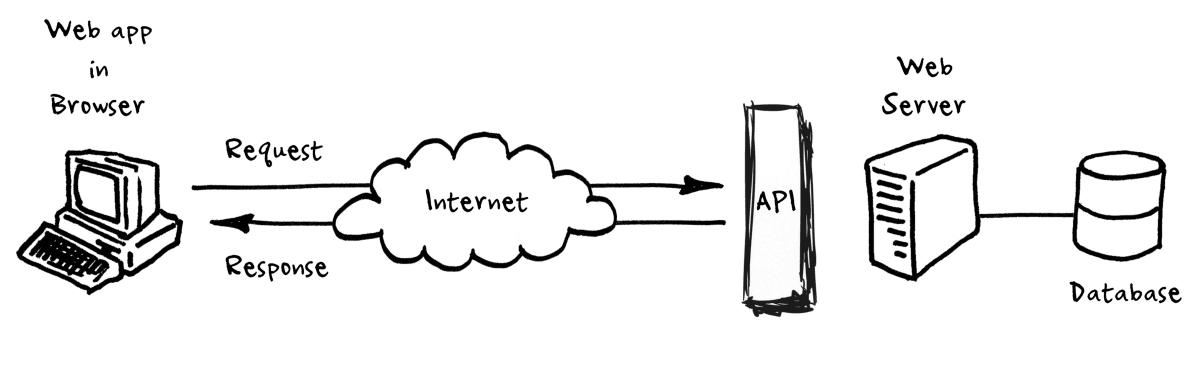
\includegraphics[width=14cm]{api.png}
\caption{Zasada działania API, źródło: wykonanie własne }
\label{Cache}
\end{figure}

% -------------------------------- 
\begin{center}
\subsection{Co to jest URI ?}
\end{center}
\textbf{URI} (ang. \emph{Uniform Resource Identifier}) to ciąg znaków identyfikujący zasób, który, na chwilą obecną, dla uproszczenia będziemy utożsamiać z~ pewną informacją. Istnieje pięć głównym charakterystyk URI:

\begin{itemize}
\item Ciąg znaków powinien być \textbf{zwięzły}, czyli nie może składać się ze spacji, tabulatorów i innych zbędnych znaków.\newline
\item Nasza informacja może być \textbf{materialna}, czyli odwoływać się do elementu świata rzeczywistego np. budynku, osoby, ale także \textbf{abstrakcyjna}, czyli odwoływać się do, przykładowo, usługi czy dokumentu sieci Web.\newline
\item Identyfikator URI jest na stałe przypisany do danego zasobu. Powinien być \textbf{stabilny}, czyli nie zmieniać się i nie znikać.\newline
\item Użytkownik może \textbf{odwołać się} do identyfikatora URI i otrzymać treściwą informację zwrotną.\newline
\item Identyfikatory dokumentów sieci Web muszą być \textbf{jednoznaczne}, czyli~ nie powinny być mylone z identyfikatorami innych zasobów.\newline
\end{itemize}
URI składa się z dwóch komponentów. Pierwszym z nich jest \textbf{URL} (ang. \emph{Uniform Resource Locator}), który odnosi się do podzbioru URI. Oprócz identyfikacji zasobów, zapewnia on środki do ulokowania zasobu i opisuje podstawowy mechanizm dostępu (np. jego "położenie" w sieci). \textbf{URN} (ang. \emph{Uniform Resource Name}) to podzbiór identyfikatorów URI, które zawierają nazwę w danej przestrzeni,\break ale nie zawierają lokalizacji. Dokumentacja mówi nam też, że każdy lokator może być też identyfikatorem, czyli \textbf{każdy URL może być URI, ale istnieją URI, które nie są URL}.

\begin{figure}[H]
\centering
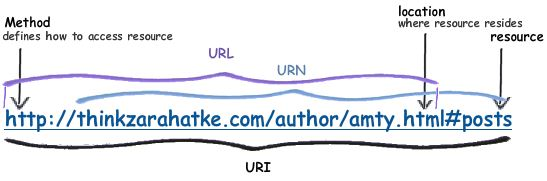
\includegraphics[width=14cm]{uri.jpg}
\caption{Zasada działania URI, URL i URN\newline
Źródło: https://prateekvjoshi.com/2014/02/22/url-vs-uri-vs-urn/}
\label{Cache}
\end{figure}

%#####################################################

\begin{center}
\subsection{Endpoints}
\end{center}
Upraszczając, \textbf{punkt końcowy} (ang. \emph{Endpoint}) to jeden koniec kanału komunikacyjnego. Gdy interfejs API współdziała z innym systemem, punkty tej komunikacji są traktowane jako punkty końcowe. W przypadku interfejsów API punkt końcowy może zawierać adres URL serwera lub usługi. Każdy punkt końcowy to lokalizacja, z której interfejsy API mogą uzyskać dostęp do zasobów potrzebnych do wykonywania swoich funkcji. Gdy interfejs API żąda informacji z aplikacji internetowej lub serwera, otrzymuje odpowiedź. Miejsce, do którego interfejsy API wysyłają żądania i gdzie znajdują się zasoby, nazywane są punktami końcowymi.

\begin{lstlisting}[
language={Python},
caption={Przykładowe Endpointy}
]
https://somewebsite.org/name/{nameId} #możemy wstawić cały link URL
/name/{nameId} #ale nie musimy
\end{lstlisting}

\newpage 
\section{REST oraz REST API}

\begin{center}
\subsection{Historia REST i REST API}
\end{center}
%#####################################################

W latach dziewięćdziesiątych nie istniały jeszcze żadne ustandaryzowane metody tworzenia API oraz ich używania. Najczęściej używanym protokołem był \textbf{SOAP} (ang. \emph{Simple Object Access Protocol}), który mimo posiadania w swej definicji słowo ,,\emph{Simple}"'', był niezwykle skomplikowany do tworzenia, przetwarzania i debugowania. Wymagał on ręcznego utworzenia pliku XML z wywołaniem \textbf{RPC} (ang. \emph{Remote Procedure Call}) w body. Po napisaniu należało sprecyzować endpoint, przesłać metodą POST definicje w~ \textbf{kopercie} (ang. \emph{SOAP envelope}) z~informacją, co znajduje się w wiadomości, dla kogo jest przeznaczona i czy jest ona obowiązkowa lub opcjonalna do danego endpointa.


\begin{lstlisting}[
language={XML},
caption={Przykładowe żądanie SOAP API}
]
<?xml version="1.0"?>
<SOAP:Envelope 
  xmins.xsi="http://www.w3.org/1999/XMLSchema/instance" 
  xmlns:xsd="http://www.w3.org/1999/XMLSchema/instance" 
  xmlns:SOAP="urn:schemas-xmlsoap-org:soap.v1">
 <SOAP:Body>
    <calculateArea>
     <origin>
      <x xsd:type="float">10</x>
      <y xsd:type="float">20</y>
     </origin>
     <corner>
      <x xsd:type="float">100</x>
      <y xsd.type="float">200<iy>
     </corner>
    </calculateArea>
  </SOAP:Body>
</SOAP:Envelope>
\end{lstlisting}

%##############################################

Wszystko zmieniło się w 2000 roku, kiedy to grupka deweloperów pod kierownictwem \textbf{Roya Feldinga} postawiła sobie za cel utworzenie standardu, pozwalającego na to, by każde dwa serwery mogły porozumiewać się pomiędzy sobą w prosty sposób. W tym samym roku, ów lider wydał rozprawę doktorską pt. ,,\emph{Architectural Styles and the Design of Network-based Software}'', która była zbiorem zasad nowej architektury nazwanej REST. Nowy standard opierał się na siedmiu głównych filarach:\newline 
\begin{itemize}
\item \textbf{Wydajność} - interakcje pomiędzy komponentami powinny być natychmiastowe.\newline
\item \textbf{Skalowalność} - umożliwiająca obsługę dużej ilości komponentów.\newline
\item \textbf{Prostota} - ujednolicenie interfejsu.\newline
\item \textbf{Modyfikowalność} - możliwość komponentów do zmian w celu sprostania zmieniającym się potrzebom.\newline
\item \textbf{Widoczność} - przejrzysta komunikacja między komponentami.\newline
\item \textbf{Przenośność} - możliwość przenoszenia kodu wraz z danymi.\newline
\item \textbf{Niezawodność} - odporność na awarie na poziomie systemu.\newline
\end{itemize}
\textbf{REST}, czyli \emph{The Representational State Transfer} jest niczym innym, jak architekturą dla systemów webowych, która prawie zawsze bazuje na protokole HTTP. Jest to zbiór pewnych dobrych praktyk, które mają działać jako drogowskaz przy tworzeniu skalowalnych aplikacji. \textbf{REST API} jest natomiast interfejsem definiującym w jaki sposób użytkownik może skomunikować się z systemem, uzyskać dostęp do zasobów, oraz w jakim formacie je otrzymuje, którego to kształt jest zdefiniowany przez architekturę REST. 

% ##################################

\section{Zasady REST}

Systemy oparte na architekturze REST nazywamy RESTful, jeżeli spełniają pewne wymagania. Systemy RESTful charakteryzują się tym, że są bezstanowe (ang. stateless) i mają mocno podkreśloną granicę pomiędzy Klientem, a Serwerem. Roy Fielding podał sześć głównych cech, które powinny zawierać systemy oparte o architekturę REST: 
 
\begin{itemize}
\item \textbf{Uniform Interface} - Serwer powinien udostępniać jednolite API, które będzie klarowne dla wszystkich systemów komunikujących się z nim. Dane powinny być w takim samym formacie i zawierać identyczny zakres. Interfejs powinien spełniać wymogi dla wielu urządzeń i aplikacji. Zasoby w~systemie powinny mieć jeden Uniform Resource Identifier, który pozwalałby na wymianę danych i powinny być łatwo dostępne przez np. HTTP request GET.
\begin{figure}[H]
\centering
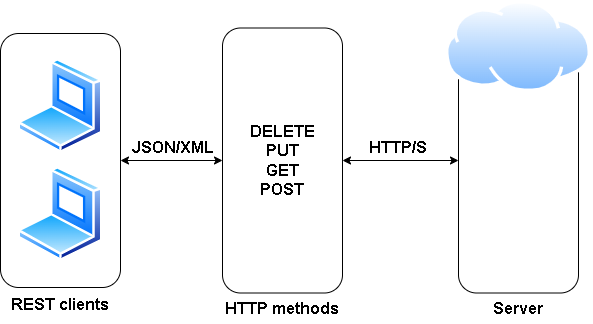
\includegraphics[width=14cm]{restarch.png}
\caption{Zasada działania REST API opartej na architekturze REST}
\label{REST API}
\end{figure}


Zasada ta zawiera jeszcze cztery reguły, który pomagają nam uprościć architekturę: 

\begin{itemize}
\item \textbf{Resource identification in requests} - Sposób reprezentacji zasobu może być różny i odłączny od samego zasobu np. serwer nie wysyła danych wprost odczytanych z bazy tylko w formacie JSON albo XML.\newline 
\item \textbf{Resource manipulation through representations} - Po otrzymaniu reprezentacji zasobów wraz z jego metadanymi od serwera, klient (jeśli ma do tego uprawnienia) może modyfikować oraz usuwać zasoby.\newline 
\item \textbf{Self-descriptive messages} - Odpowiedź serwera powinna zawierać wystarczającą ilość informacji, aby serwer mógł ją obsłużyć np. poprzez wartość ,,media type''(inaczej ,,MIME type'').\newline 
\item \textbf{Hypermedia as the engine of application state} (HATEOAS) - HATEOAS jest ograniczeniem architektury aplikacji REST, która sprawia, że architektura stylu RESTful jest inna od większości innych architektur. Termin ,,hypermedia'' odnosi się do wszelkich treści zawierających łącza do innych form mediów, takich jak obrazy, filmy i teksty. Styl architektoniczny REST pozwala nam używać linków hipermedialnych w treści odpowiedzi. Pozwala klientowi dynamicznie przechodzić do odpowiednich zasobów korzystając z łącz hipermedialnych. Najlepiej zobrazować to na przykładzie Graph API od Facebooka np. korzystając z przykładowej odpowiedzi znajdującej się w dokumentacji. Niektóre wartości zostały skrócone dla przejrzystości: 


\begin{lstlisting}[
caption={Odpowiedź od Graph API}, basicstyle=\ttfamily\scriptsize
]
{
   "feed":{
      "data":[
         {
            "created_time":"2017-12-12T01:24:21+0000",
            "message":"This picture is nice",
            "id":"820882001277849_1809387339093972"
         },
         {
            "created_time":"2017-12-11T23:40:17+0000",
            "message":":)",
            "id":"820882001277849_1809316002434439"
         },
         {
            "created_time":"2017-12-11T23:31:38+0000",
            "message":"Thought you might enjoy this",
            "id":"820882001277849_1809310929101613"
         }
      ],
      "paging":{
         "cursors":{
            "before":"Q2c4U1pXNTBYM0YxWlhKNVgzTjBiM0",
            "after":"Q2c4U1pXNTBYM0YxWlhKNVgzTjBiM0"
         },
         "next":"https://graph.facebook.com/820882001277849/feed?access_token"
      }
   },
   "id":"820882001277849"
}
\end{lstlisting}

W sekcji paging, pod kluczem next widnieje link, który poprowadzi nas do kolejnych wyników.\newline 
\end{itemize}

\item \textbf{Client-Serwer} - Projektując, a następnie implementując aplikacje klienta i~serwera należy wyznaczyć widoczną granicę pomiędzy oba programami. Oznacza to, że klient i serwer mogą rozwijać się bez ingerencji pomiędzy sobą. Zamysł ten pomaga w realizacji ww. Uniform Interface, a także zwiększa możliwości skalowania i rozszerzalności, a obsługa błędów jest znacznie łatwiejsza. Jeżeli na przykład dokonamy zmiany w aplikacji pisanej dla systemu iOS (to będzie nasz klient), to zmiana ta nie powinna w żaden sposób wpływać na aplikacje serwerową (strukturę bazy danych i tym podobne). Tak samo powinno to działać w drugą stronę. 


\begin{figure}[H]
\centering
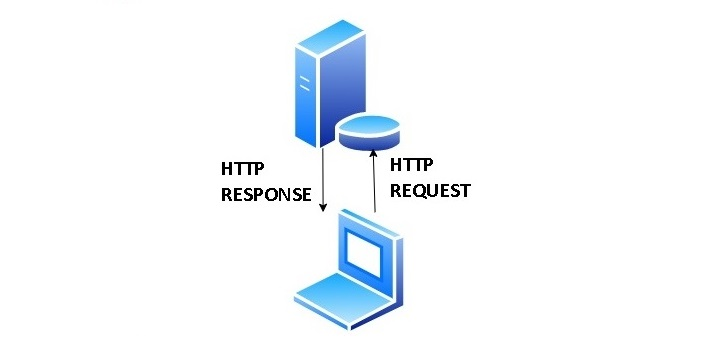
\includegraphics[width=14cm]{rest.jpg}
\caption{REST w prosty sposób pomaga deweloperom w planowaniu interakcji pomiędzy niezależnymi systemami}
\label{REST}
\end{figure}

%###################################################

\item \textbf{Stateless} - według tego założenia wszystkie interakcje pomiędzy klientem, a serwerem powinny być bezstanowe. Oznacza to, iż serwer nie zapisuje żadnych stanów aplikacji klienta, a jedynie przetwarza informacje wysyłane przez niego. Każde żądanie powinno być przetwarzane jako nowe i zawierać komplet informacji. Jeżeli klient musi być stanowy, jak np. przy logowaniu, to każde żądanie powinno zawierać tylko potrzebne informacje, wraz z danymi do autoryzacji i uwierzytelniania.\newline 
\item \textbf{Cacheable} - odpowiedź, którą użytkownik otrzyma z REST API musi jasno definiować, czy ma ona być cacheable czy non-cacheable. Ma to znaczenie przy danych, które bardzo szybko stają się nieaktualne oraz przy danych, które aktualizują się relatywnie rzadko – nie ma sensu na przykład cacheować współrzędnych geograficznych pędzącego samolotu, natomiast jego kolor czy nazwę już tak.\newline
\item \textbf{Layered System} - REST pozwala na odseparowanie warstw. Możemy wdrożyć nasze API na serwer A, przechowywać dane na serwerze B i przetwarzać żądania na serwerze C. Klient nie wie o zewnętrznych usługach i serwisach, z których korzysta serwer. Pozwala to na rozbicie serwisu na wiele mikroserwisów, które można łatwo aktualizować. Dzięki temu zachowujemy transparentność i separację logiki od warstwy WWW. Niestety takie rozwiązanie ma pewne wady, ponieważ może wprowadzać opóźnienia przez potrzebę komunikacji pomiędzy różnymi częściami naszej aplikacji.\newline
\item \textbf{Code-On-Demand} - jest to zasada, która jest opcjonalna, ponieważ prawie zawsze będziemy wysyłać dane w statycznej formie, jak np. XML albo JSON. Nasz serwis może wysyłać gotowe fragmenty kodu np. skrypty JavaScript do ich przetworzenia. 
\end{itemize}
%####################################################################

\section{Podstawowy element REST API, czyli zasoby}

\begin{quote}{Roy Fielding}
The key abstraction of information in REST is a resource. Any information that can be named can be a resource: a document or image, a temporal service (e.g. ,,today’s weather in Los Angeles''), a collection of other resources, a non-virtual object (e.g., a person), and so on. In other words, any concept that might be the target of an author’s hypertext reference must fit within the definition of a resource. A resource is a conceptual mapping to a set of entities, not the entity that corresponds to the mapping at any particular point in time.
\end{quote}

\begin{center}
\subsection{Czym jest zasób?}
\end{center}

\textbf{Zasób} (ang. \emph{Resource}) jest elementarną częścią REST API. Wykorzystujemy go właśnie podczas interakcji z API. Czym więc jest zasób? Nie jest łatwo odpowiedzieć na to pytanie, ponieważ zasób to pojęcie abstrakcyjne. Dowolna informacja, która może posiadać nazwę, może być zasobem. Dlatego też przyjęto kilka podstawowych kryteriów, by można było nazwać daną informację zasobem:\newline


\begin{itemize}
\item Musi być rzeczownikiem.
\item Musi być unikatowa, czyli definiować konkretną rzecz i być jak najbardziej sprecyzowana. Przykładowo, budynek nie jest zasobem, ponieważ jest zbyt ogólny, lecz biblioteka już nim jest. 
\item Musi być możliwa do przedstawienia w formie danych.
\item Music posiadać przynajmniej jeden adres URI, pod którym jest dostępny. URI jednocześnie jest nazwą, jak i adresem zasobu.\newline
\end{itemize}


\begin{center}
\subsection{Nazewnictwo}
\end{center}

Odpowiednie nazewnictwo i struktura informacji pozwala na zwiększenie użyteczności oraz elastyczności, ułatwiając rozbudowę i modyfikację aplikacji. Niestety sposób nazywania zasobów jest kwestią bardzo dyskusyjną i nie istnieje jedna zasada jak powinniśmy poprawnie nazywać zasoby. Jednakże istnieją wskazówki, które można zastosować:\newline
\begin{itemize}
\item \textbf{Obiekty vs. Akcje} - Zasoby powinny być tak zaprojektowane by były odłączne od akcji. Dzięki temu możemy wykonywać wiele akcji na pojedynczym zasobie. Przytoczę taki przykład:\newline

\begin{lstlisting}[
language={Python},
caption={Przykład pierwszy}
]
GET /users # Gets list of all users
POST /users # Adds new user
DELETE /users # Deletes all users
\end{lstlisting}

\begin{lstlisting}[
language={Python},
caption={Przykład drugi}
]
GET /getUsers # Gets list of all users
POST /addUsers # Adds new user
DELETE /users/delete # Deletes all users
\end{lstlisting}

Pierwszy z powyższych przykładów posiada jeden zasób users, na którym wykonujemy różne akcje z wykorzystaniem metod HTTP, czyli mamy jeden zasób na którym wykonujemy wiele akcji. Natomiast przykład drugi posiada trzy różne adresy, które są połączone z akcją wykonywaną w naszej aplikacji. Jednoznacznie widać, że założenia z przykładu drugiego mocno odbiegają od naszych założeń REST, ponieważ powiązanie API z naszą aplikacją uniemożliwia rozwijanie się aplikacji, jak i API niezależnie od siebie.\newline
\item \textbf{Rzeczowniki vs. Czasowniki} - jednym ze sposobów weryfikacji, czy zasób jest odłączony od akcji, jest użycie samego rzeczownika w nazwie. Jeśli w adresie URI zasobu znajduje się czasownik, np. /getUsers lub /addUsers, to możemy podejrzewać że ten zasób jest bardzo mocno powiązany z konkretną akcją.\newline
\item \textbf{Liczba pojedyncza vs. Liczba mnoga} - starajmy się używać liczby mnogiej przy nazewnictwie zasobów, np. /users zamiast /user. Zwiększa to czytelność naszego API, jednakże ta zasada jest bardzo dyskusyjna. Obiektywnie nasze API powinno być zbudowane konsekwentnie i spójnie. 
\end{itemize}
% ######################################################################

\begin{center}
\section{Model dojrzałości Richardsona}
\end{center}

Jako, że REST jest tylko zbiorem wytycznych i dobrych rad dla tworzenia API, to deweloperzy mają bardzo dużą elastyczność do definiowania jak bardzo ``REST-owe`` będzie ich API. Zakładając sytuację, że napiszemy prostą aplikację RESTful API, to skąd możemy mieć pewność, że jest ona w stylu REST? Można powiedzieć, że skoro wykorzystujmy protokół HTTP i używamy formatu danych JSON, to serwis jest RESTful. \textbf{Model dojrzałości Richardsona}(ang. \emph{Richardson Maturity Model}) pozwala ocenić w jakim stopniu aplikacja jest RESTful. Model definiuje 4 poziomy (0-3) i zakłada, że \textbf{każde API należy do jednego z czterech poziomów dojrzałości}.

\begin{itemize}
\item \textbf{Poziom 0} - Na poziomie zerowym modelu dojrzałości znajdują się aplikacje, które nie spełniają założeń architektury REST. Protokół HTTP wykorzystywany jest tylko jako warstwa transportowa. Używane są tylko metody GET i POST oraz status zwracany zawsze jest 200 OK. Nie ma unikalnych adresów dla zasobów. Do tego poziomu zaliczamy np. protokoły SOAP i RPC.

\begin{lstlisting}[
language={Python},
caption={Przykładowe API dla poziomu 0}
]
POST /api/findSomething
POST /api/updateSomething
\end{lstlisting}

\begin{lstlisting}[
language={Python},
caption={Dodawanie np. rzeczy}
]
POST /api/addSomething HTTP/1.1
{ "item_name":"Chair" }
\end{lstlisting}

\newpage 
\begin{lstlisting}[
language={Python},
caption={Odpowiedzi}
]
200 OK
{ "item_id":50 }
# or
200 OK
{ "error":"Wrong data input." }
\end{lstlisting}

\item \textbf{Poziom 1} - Na pierwszym poziomie modelu dojrzałości wykorzystywanych jest wiele identyfikatorów URI, jednakże używa się podstawowych metod HTTP, jak np. GET, czy POST. Na tym poziomie mamy już zdefiniowane zasoby, które powinny posiadać indywidualny identyfikator URI. Zasób nie powinien być dostępny pod wieloma adresami, tzn. musi mieć unikalny adres.

\begin{lstlisting}[
language={Python},
caption={Przykładowe API dla poziomu 1}
]
POST /api/something/id/get
POST /api/something/create
\end{lstlisting}

\item \textbf{Poziom 2} - Drugi poziom modelu dojrzałości rozszerza podstawowe metody HTTP o dodatkowe, jak np. PUT, PATCH i DELETE. Dodane metody używane są zgodnie z ich przeznaczeniem.

\begin{lstlisting}[
language={Python},
caption={Przykładowe API dla poziomu 2}
]
POST /api/something
GET /api/something/item_id
PUT /api/something/item_id
PATCH /api/something/item_id
DELETE /api/something/item_id
\end{lstlisting}

Drugi poziom wprowadza też rozszerzenie dla statusów odpowiedzi. Statusy należy wykorzystywać zależnie od sposobu realizacji zapytania.\\

\begin{itemize}
\item 1XX – Kody informacyjne
\item 2XX – Kody powodzenia
\item 3XX – Kody przekierowania
\item 4XX – Kody błędu aplikacji klienta
\item 5XX – Kody błędu serwera
\end{itemize}

\newpage 
\begin{lstlisting}[
language={Python},
caption={Dodawanie np. rzeczy}
]
POST /api/addSomething HTTP/1.1
{ "item_name":"Chair" }
\end{lstlisting}

\begin{lstlisting}[
language={Python},
caption={Odpowiedzi}
]
201 Created
{ "item_id":50 }
# or
409 Conflict
{ "error":"Wrong data input." }
\end{lstlisting}

\item \textbf{Poziom 3} - Trzeci poziom (najwyższy) wymaga implementacji HATEOAS. HATEOAS zarządza interakcją dla klienta. Klient nie zna wszystkich punktów końcowych API dla danych żądań.

\begin{lstlisting}[
language={Python},
caption={Przykład pobierania osoby o identyfikatorze 36:}
]
GET /api/persons/36 HTTP/1.1
\end{lstlisting}

\begin{lstlisting}[
language={Python},
caption={Przykładowa odpowiedź:}
]
HTTP/1.1 200 OK
{ "id":36, "name":"Damian Kuich", "age":23,
"link":{"address":"/api/addresses/43"} }
\end{lstlisting} 

\end{itemize}

\section{Django}
\textbf{Django} jest frameworkiem typu open-source,  bazującym na języku Python, który w bardzo prosty sposób umożliwia tworzenie skalowalnych i szybkich aplikacji webowych. Operuje on na modelu architektonicznym \textbf{MTV}(ang. \emph{Model-Template-Views}). 

\begin{figure}[H]
\centering
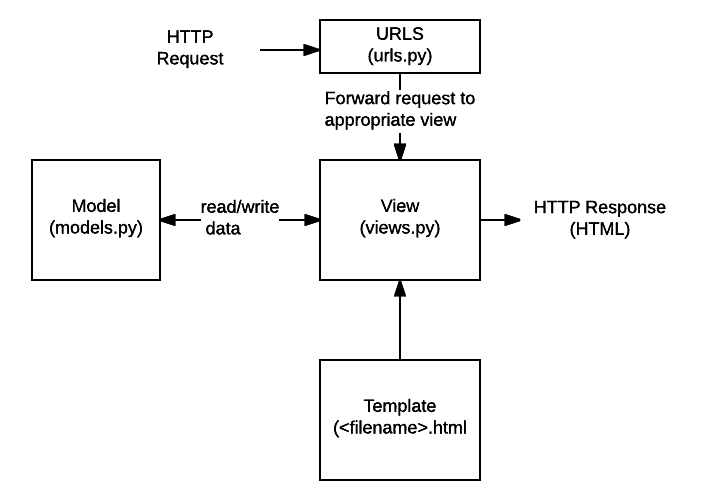
\includegraphics[width=14cm]{mtv.png}
\caption{Architektura MTV\newline
Źródło: https://developer.mozilla.org/en-US/docs/Learn/Server-side/Django/Introduction}
\label{MTV}
\end{figure}

\begin{center}
\subsection{URLs}
\end{center}
Chociaż możliwe jest przetwarzanie żądań z każdego adresu URL za pośrednictwem jednej funkcji, znacznie łatwiej jest napisać oddzielny widok (ang. \emph{View}) do obsługi wielu zasobów. URLs służy do przekierowywania żądań HTTP do odpowiedniego widoku na podstawie adresu URL. Narzędzie odwzorowujące adresy URL może również dopasować określone wzorce ciągów lub cyfr, które pojawiają się w adresie URL, i przekazać je dalej jako dane.

\begin{center}
\subsection{Views}
\end{center}
View służy do przetwarzania żądań i odpowiedzi HTTP. Pobiera dane potrzebne do wykonania żądań z pomocą modeli (ang. Models), jak i formatują odpowiedzi do szablonów (ang. Templates).


\begin{center}
\subsection{Models}
\end{center}
Modele to obiekty, które kształtują strukturę danych aplikacji. Umożliwiają wykonywanie na danych operacji, takich jak usuwanie, dodawanie, czy modyfikowanie. 


\begin{center}
\subsection{Templates}
\end{center}
Szablony to pliki tekstowe definiujące strukturę lub układ pliku (na przykład strony HTML), z symbolami zastępczymi używanymi do reprezentowania rzeczywistej zawartości. Widok może dynamicznie tworzyć stronę HTML przy użyciu szablonu HTML, wypełniając ją danymi z modelu. Szablon może służyć do definiowania struktury dowolnego typu pliku nie tylko HTML.
\section{Django REST Framework}
\textbf{Django REST Framework} jest frameworkiem typu open-source napisanym w języku Python. Pozwala on na implementacje architektury REST do naszego API, co umożliwia nam utworzenie RESTful API. Opiszmy więc, jak została zaimplementowana architektura REST do tego frameworka, przechodząc przez jej główne założenia z rozdziału 2.3.
\begin{center}
\subsection{Unifrom Interface}
\end{center}
Unifrom Interface zakłada ujednolicenie API i danych, by były one klarowne dla innych serwisów. Powinno to oznaczać, że system powinien posiadać jeden główny URI dzięki, któremu~ byśmy mogli korzystać z metod HTTP. Django REST Framework pomaga w budowaniu interfejsu API REST poprzez tworzenie punktów końcowych za pomocą widoków ogólnych. Te ogólne widoki pomagają stworzyć pełny punkt końcowy CRUD (create, read, $\dots$) w modelu Django przy niewielkim wysiłku. Utworzony punkt końcowy jest zgodny z interfejsem API Rest struktury adresu URL dla zasobu. 

\newpage 
\begin{center}
\subsection{HATEOAS}
\end{center}
To czego REST nie potrafi, to dostarczenie czytelnych dla maszyny formantów hypermedialnych takich jak HAL, Collection+JSON, JSON API lub mikroformantów HTML w sposób domyślny. Nie udostępnia również możliwości automatycznego stworzenia pełnego API HATEOAS zawierającego opisy formatów i semantycznie oflagowanych hiperlinków. Dla osiągnięcia takiego efektu musiałyby zostać podjęte decyzje wykraczające poza obszar frameworka. 
\begin{center}
\subsection{Client-Server}
\end{center}
Już sama esencja tego, że Django REST Framework pozwala utworzyć backend serwera, który nie jest częścią interfejsu użytkownika aplikacji, jest istotą architektury klient-serwer. Każda aplikacja, którą tworzymy za pomocą Django Rest Framework posiada API, które jest zupełnie oddzielne od API klienta. 
\begin{center}
\subsection{Stateless}
\end{center}
Django REST Framework dzięki interfejsowi WSGI/ASGI nie musi zapisywać żadnych informacji ani polegać na nich. Poniżej zobrazowano skróconą zasadę działania:



\begin{lstlisting}[
language={Python},
caption={Przykład kodu stateless, gdzie nie zapisujemy żadnych danych:}]
while True:
    request = io.listen_for_request()
    response = handle_request(request)
return response
\end{lstlisting}

\begin{center}
\subsection{Cacheable}
\end{center}
Django REST Framework ma wbudowane narzędzia do Cachowania.

\newpage
\begin{center}
\subsection{Layered System}
\end{center}
Django zapewnia wiele interesujących połączeń między warstwami, a użycie go dla wszystkich warstw pozwala wykorzystać te połączenia. Przykładowo, użycie Django ORM oznacza, że otrzymujemy świetną aplikację administracyjną. Możemy wybrać inny ORM, ale nie dostaniemy wraz z nim aplikacji administratora. Django, też nie utrudnia rozbicia naszego serwisu na wiele pomniejszych mikroserwisów. 
\begin{center}
\subsection{Code-On-Demand}
\end{center}
Django umożliwia na rozszerzenie funkcjonalności szablonów do wysyłania np. formularzy jako endpoint.
\section{Podsumowanie}
W pracy przedstawiono podstawowe zagadnienia związane z API. Omówiono także główne cechy i zasady REST. Zwrócono uwagę na to, co sprawia, że API jest RESTful. Wspomniano też o ewolucji API dzięki modelowi dojrzałości Richardsona. Na końcu ponownie przedstawiono główne założenia architektury REST, jednakże tym razem dla stwierdzenia czy Django REST Framework naprawdę pozwala na tworzenie prawdziwego RESTful API. Po przeanalizowaniu implementacji głównych paradygmatów REST w Django REST Framework, czy nawet w samym Django, można wywnioskować, że umożliwia on tworzenie API zgodnie z REST.

%###############################################################
\chapter{Integracja projektu opartego o Django z bazą danych PostgreSQL}
Baza danych to zbiór informacji, danych, zazwyczaj przechowywanych w~formie elektronicznej w systemie komputerowym.  
Dane umieszczone są w wierszach i kolumnach wielu tabel, dzięki czemu przetwarzanie ich oraz tworzenie zapytań ich dotyczących odbywa się w zorganizowany i sprawny sposób. W~dzisiejszych czasach większość baz danych wykorzystuje język SQL (Structured Query Language), czyli strukturalny język zapytań. 
SQL to język programowania używany do tworzenia zapytań dotyczących danych. Jest wykorzystywany przez niemal wszystkie relacyjne bazy danych. Został on opracowany w latach 70-tych przez firmę IBM. Przy tworzeniu języka brała udział firma Oracle, czego efektem było wprowadzenie standardu SQL ANSI i powstanie wielu rozszerzeń języka SQL.  
Istnieje wiele typów baz danych. Oto kilka z nich:  

\begin{itemize}
\item Relacyjne bazy danych
\item Obiektowe bazy danych
\item Rozproszone bazy danych
\item Hurtownie danych
\item Bazy danych NoSQL
\item Grafowe bazy danych
\end{itemize}

Bazy danych obsługiwane są przez system zarządzania DBMS (Database Management System). Stanowi on swego rodzaju pomost między danymi a~programami wykorzystującymi te dane lub użytkownikami końcowymi. Dzięki niemu można pobierać, aktualizować informacje oraz konfigurować sposób, w~jaki są one zorganizowane. System pozwala również na wykonywanie zadań administracyjnych, takich jak tworzenie oraz przywracanie kopii zapasowych.
W pracy krótko przedstawiono cztery systemy zarządzania bazami danych: 

\begin{itemize}
\item MySQL 
\item MS SQL Server 
\item Oracle 
\item PostgreSQL 
\end{itemize}
\section{MySQL}
MySQL to darmowy i otwarty system zarządzania relacyjnymi bazami danych (RDBMS). Jego właścicielem jest Oracle, który oferuje płatne wersje premium MySQL z dodatkowymi usługami. Jest to lekka baza danych, która może być instalowana i używana przez programistów na serwerach aplikacji produkcyjnych z dużymi aplikacjami wielowarstwowymi, a także na komputerze stacjonarnym. Jest bezpieczny i nie jest podatny na żadne luki w zabezpieczeniach. MySQL oferuje obsługę następujących języków: C/C++, Delphi, Java, Lisp, Node.js, Perl, PHP, R.
MySQL oferuje obsługę w chmurze, instalacje lokalne oraz jest kompatybilny z następującymi systemami operacyjnymi i formatami: Windows, MacOS, Linux (Ubuntu, Debian, Generic, SUSE Linux Enterprise Server, Red Hat Enterprises, Oracle), Oracle Solaris, Fedora, FreeBSD.


\begin{table}[H]
\caption{Wady i zalety MySQL}
\label{tabela-MySQL}
\centering
\begin{adjustbox}{width=1\textwidth}
\small
\begin{tabular}{lr}
\toprule
Zalety & Wady\\
\midrule
Ochrona danych & Złożona logika biznesowa\\
Skalowalność na żądanie & Kilka problemów ze stabilnością\\
Całodobowa dostępność & Transakcje nie są obsługiwane zbyt wydajnie\\
Kompleksowe wsparcie transakcyjne & Funkcjonalność zależna od dodatków\\
Pełna kontrola przepływu pracy & Wcześniejsza wiedza jest koniecznością\\
Elastyczność open source &\\
Szerokie zastosowanie i łatwe w użyciu &\\
Szybki, przenośny i bezpieczny & Konieczna jest znajomość tematu\\
\bottomrule
\end{tabular}
\end{adjustbox}
\end{table}
\section{MS SQL Server}
MS SQL Server to relacyjny system zarządzania bazami danych (RDBM) opracowany i obsługiwany przez firmę Microsoft. Używa wariantu \emph{Structured Query Language} (SQL) o nazwie T-SQL. Zwykle zawiera silnik relacyjnej bazy danych, który przechowuje dane w tabelach, kolumnach i wierszach,  \emph{Integration Services} (SSIS), które są narzędziem do przenoszenia danych do importowania, eksportowania i przekształcania danych. W jego skład wchodzą również \emph{Reporting Services} (SSRS), które służą do tworzenia raportów i udostępniają je użytkownikom końcowym, a także  \emph{Analysis Services} (SSAS), czyli wielowymiarowa baza danych służąca do wykonywania zapytań o dane z głównego silnika.
MS SQL Server oferuje obsługę języków programowania takich jak: C\#, C++, Delphi, Go, Java, JavaScript, PHP, Python, R, Ruby , Visual Basic.
MS SQL Server jest dostępny na systemach Microsoft Windows oraz Linux.

\begin{table}[H]
\caption{Wady i zalety MS SQL Server}
\label{tabela-MS SQL Server}
\centering
\begin{adjustbox}{width=1\textwidth}
\small
\begin{tabular}{lr}
\toprule
Zalety & Wady\\
\midrule
Dostępna wersja darmowa systemu & Kosztowna wersja dla przedsiębiorstw\\
Wysokie bezpieczeństwo danych & Ograniczona kompatybilność\\
Łatwość konfiguracji & Kilka problemów ze stabilnością\\
Łatwość konfiguracji & \\
Wsparcie odzyskiwania danych & \\
\bottomrule
\end{tabular}
\end{adjustbox}
\end{table}
\section{Oracle}
Oracle to system zarządzania relacyjnymi bazami danych wydany w 1980 roku z podstawowymi funkcjami SQL, który sam się steruje, zabezpiecza, samo naprawia i eliminuje podatne na błędy ręczne zarządzanie bazą danych. Umożliwia bezpieczne przechowywanie i szybkie pobieranie danych. Oracle to pierwsze narzędzie bazodanowe opracowane w celach biznesowych, do zarządzania danymi za pomocą języka zapytań.
Oracle oferuje obsługę języków programowania takich jak: C, C\#, C++, Delphi, Haskell, Java, JavaScript, C, Perl, PHP, Python, R, Ruby, Visual Basic.
Oracle jest dostępny dla następujących systemów operacyjnych: Windows, Mac OS X, Linux, UNIX, z/OS.

\begin{table}[H]
\caption{Wady i zalety MySQL}
\label{tabela-Oracle}
\centering
\begin{adjustbox}{width=1\textwidth}
\small
\begin{tabular}{lr}
\toprule
Zalety & Wady\\
\midrule
Wszechstronność & Trudny do nauczenia i obsługi\\
Kompatybilność ze składnią SQL i PL & Wysoki koszt obsługi\\
Poprawiona wydajność & Składniki zapytań poza standardem ANSI \\
Grupowanie transakcji & Intensywne obciążenie sprzętu\\
\bottomrule
\end{tabular}
\end{adjustbox}
\end{table}
\section{PostgreSQL}
PostgreSQL to darmowy i otwarty system zarządzania obiektowo-relacyjnymi bazami danych (ORDBMS). Obecnie zarządzany jest przez społeczność programistów, która pomaga ułatwić i przyspieszyć  pracę wszystkich użytkowników.
PostgreSQL zapewnia zarówno obiektową, jak i relacyjną funkcjonalność bazy danych. Był pierwszym systemem DBMS, który zaimplementował funkcje kontroli współbieżności wielu wersji (MVCC). Jest obecnie uważany za najbardziej zaawansowany silnik bazy danych. Obsługuje tekst, obrazy, dźwięki i wideo oraz zawiera interfejsy programistyczne dla wielu języków. PostgreSQL może być rozszerzany przez użytkownika na wiele sposobów.
PostgreSQL oferuje obsługę nieco szerszej gamy języków: C/C++, Delphi, Erlang, Go, Java, JavaScript, Lisp, .Net, Python, R, Tcl.
PostgreSQL jest dostępny dla następujących systemów operacyjnych: MacOS, Solaris, Windows, BSD (FreeBSD, OpenBSD), Linux, CentOS, Fedora, Scientific, Oracle, Debian, Ubuntu Linux i pochodne.


\begin{table}[H]
\caption{Wady i zalety PostgreSQL}
\label{tabela-PostgreSQL}
\centering
\begin{adjustbox}{width=1\textwidth}
\small
\begin{tabular}{lr}
\toprule
Zalety & Wady\\
\midrule
Wysoce skalowalny & Stosunkowo niska prędkość czytania\\ 
Posiada wiele interfejsów & Optymalna konfiguracja może być kłopotliwa\\ 
Obsługuje JSON &  \\ 
Szerokie możliwości rozbudowy &  \\ 
Przetwarzanie złożonych typów danych &  \\ 
Elastyczne wyszukiwanie pełno tekstowe  &  \\ 
Wieloplatformowy &  \\ 
Zdolny do obsługi danych w TB &  \\ 
\bottomrule
\end{tabular}
\end{adjustbox}
\end{table}
  

W projekcie składającym się na praktyczną część pracy, zastosowany został PostgreSQL. Jednym w głównych czynników wpływających na wybór był fakt, że PostgreSQL oferowany jest poprzez używaną podczs wdrożenia platformę chmurową Heroku. 
\section{Łączenie z bazą danych PostgreSQL}
Integracja Django z PostgreSQL rozpoczyna się od stworzenia nowej bazy lub połączenia z obecnie istniejącą.
Domyślnie Django jest skonfigurowane do używania \texttt{SQLite} jako swojego zaplecza, dlatego wymagana jest lekka zmiana zawartości pliku settings.py tak, aby używanie Postgresa było możliwe. 

Poniżej znajduję się kod~\ref{databases} potrzebny do połączenia się bazą danych oferowaną przez Heroku.  
\begin{lstlisting}[
language={Python},
xleftmargin=14pt,
caption={Fragment pliku \texttt{settings.py}},
label={databases}
]
DATABASES = {,  
	'default': { 
	'ENGINE': 'django.db.backends.postgresql', 
	'NAME': '', 
	'USER': '', 
	'PASSWORD': '', 
	'HOST': 'ec2-54-160-18-230.compute-1.amazonaws.com', 
	'PORT': '5432', 
	} 
} 
\end{lstlisting}
\section{Modele}

Wyjściowo baza implementuje podstawowe schematy danych takie jak  \texttt{Users} oraz \texttt{Groups}. Aby zawierała inne dane, potrzebne jest zdefiniowanie ich we frameworku, w pliku \texttt{models.py}.
Najważniejszą częścią modelu są zdefiniowane pola bazy danych, będące instancja klasy \texttt{Field}. Są to na przykład: \texttt{CharField}, \texttt{TextField}, \texttt{ForeignKey}, \texttt{IntegerField}, \texttt{BooleanField}, \texttt{DateTimeField}.

Pola modeli przeznaczone dla PostgreSQL (django.contrib.postgres.fields):

\begin{itemize}
	\item \texttt{ArrayField} - pole do przechowywania list danych.
	\item \texttt{HStoreField} - pole do przechowywania par klucz:wartość. W Pythonie typ danych reprezentowany jako dict.
	\item \texttt{JSONField} - pole do przechowywania danych zakodowanych w formacie \texttt{JSON}.
	\item \texttt{IntegerRangeField} - pole przechowuje zakres liczb całkowitych.
	\item \texttt{BigIntegerRangeField} - pole przechowuje zakres dużych liczb całkowitych.
	\item \texttt{DecimalRangeField} - pole przechowuje zakres wartości zmiennoprzecinkowych.
	\item \texttt{DateTimeRangeField} - pole przechowuje szereg sygnatur czasowych.
	\item \texttt{DateRangeField} - pole przechowuje zakres dat.
\end{itemize}

Każde pole określone jest poprzez argumenty. Przykładowo pole \texttt{CharField} wymaga podania argumentu \texttt{max\_length}, który określa maksymalną ilość znaków. Każde pole posiada również zestaw ogólnodostępnych argumentów np.: \texttt{null (True/False)}, \texttt{blank (True/False)}, \texttt{default}, \texttt{unique (True/False)}.

\begin{lstlisting}[
language={Python},
xleftmargin=14pt,
caption={Fragment pliku models},
label={models}
]
class Section(models.Model):
    section_name = models.CharField(max_length=500,unique=True)

    def __str__(self):
        return self.self_name()

    def self_name(self):
        return self.name

class Skill(models.Model):
    skill_name = models.CharField(max_length=500,unique=True)
    section = models.ForeignKey(Section, on_delete=models.CASCADE)
	  # ...
        return self.skill_name

class Task(models.Model):
    TYPES = {
        (1, "Otwarte"),
        (2, "Zamknięte"),
    }
    LEVELS = {
        (1, "Podstawowy"),
        (2, "Rozszerzony"),
    }
    text = models.CharField(max_length=600,unique=True)
    wrong_answers =ArrayField(models.CharField(
				max_length=200), blank=True)
    correct_answers =ArrayField(models.CharField(
				max_length=200), blank=True)
    task_type = models.IntegerField(choices=TYPES)
    level = models.IntegerField(choices=LEVELS)

	  # ...
        return self.text


class TestJSON(models.Model):
    name = models.TextField(null=True)
    tasks = JSONField(null=True)

    # ...
        return self.name
\end{lstlisting}

Powyższy przykład~\ref{models} obrazuje definicje modeli \texttt{Skill}, \texttt{Section}, \texttt{Task} oraz \texttt{TestJSON}, 
które odpowiadają zadaniu, działom wraz z umiejętnościami oraz obiektu testu w Generatorze Sprawdzianów. 
Model \texttt{Task} zawiera m.in. pola wrong\_answers oraz correct\_answers będące polami typu \texttt{ArrayField}. Pola te przeznaczone
są do przechowywania poprawnych oraz niepoprawnych odpowiedzi na pytania zamknięte. Odpowiedzi może być wiele, dlatego z~pomocą
przychodzi \texttt{ArrayField}, czyli lista obiektów. W tym przypadku są to obiekty typu tekstowego.
Model \texttt{TestJSON} zawiera m.in. pole tasks, zawierające wszystkie zadania w formacie JSON przypisane do danego testu.
Dzięki temu każdy użytkownik może dodawać do testu zadanie z naszej bazy, a następnie edytować je według własnego uznania bez ingerencji
w oryginał.
Na końcu każdego modelu dodana została jego reprezentacja, przez co w zakładce admin widoczna będzie nazwa obiektu, co w znacznym stopniu ułatwi jego identyfikację.

\section{Migracje}
Po zdefiniowaniu modelu, wymagane jest wykonanie migracji. Migracje to sposób Django na propagowanie zmian schematu bazy danych takich jak dodawanie pola, edytowanie, usuwanie modelu itp. Są zaprojektowane w taki sposób, aby były w większości automatyczne, jednak wymagane jest ich tworzenie w taki sposób, aby uniknąć powstania błędów. \emph{Makemigrations} jest odpowiedzialne za pakowanie zmian w modelu do indywidualnych plików migracyjnych, z kolei \emph{migrate} jest odpowiedzialny za stosowanie ich w bazie danych.
Niektóre bazy danych są bardziej wydajne niż inne, biorąc pod uwagę migrację schematów. PostgreSQL cechuje się wysoką wydajnością pod względem obsługi schematów, natomiast MySQL nie obsługuje transakcji zmiany schematu. Jeżeli dana migracja się nie powiedzie, zmuszeni jesteśmy ręcznie cofnąć zmiany, a następnie spróbować ponownie. 

Aby zbudować tabele w bazie danych, wykonujemy migrację i uruchamiany ją poniższymi poleceniami: 

\begin{lstlisting}[style=DOS]
>python manage.py makemigrations
>python manage.py migrate
\end{lstlisting}
Po wykonaniu migracji, Django wprowadzi do bazy danych następujące polecenie.
\begin{lstlisting}[
language={SQL},
caption={SQL dla modelu Task, Skill oraz Section},
label={sql}
]
CREATE TABLE "section" (
	"id" serial NOT NULL PRIMARY KEY, 
	"section_name" varchar(500) NOT NULL UNIQUE);

CREATE TABLE "skill" (
	"id" serial NOT NULL PRIMARY KEY, 
	"skill_name" varchar(500) NOT NULL UNIQUE, 
	"section_id" integer NOT NULL);

CREATE TABLE "task" (
	"id" serial NOT NULL PRIMARY KEY, 
	"text" varchar(600) NOT NULL UNIQUE, 
	"wrong_answers" varchar(200)[] NOT NULL, 
	"correct_answers" varchar(200)[] NOT NULL,
	"task_type" integer NOT NULL, 
	"level" integer NOT NULL, 
	"private" boolean NOT NULL, 
	"points" integer NOT NULL, 
	"author_id" integer NOT NULL);

CREATE TABLE "task_skill" (
	"id" serial NOT NULL PRIMARY KEY, 
	"task_id" integer NOT NULL, 
	"skill_id" integer NOT NULL);
	# ...
\end{lstlisting}

Porównując wycinek~\ref{models} z poleceniem~\ref{sql} zauważyć można, że w pliku models.py nie został zdefiniowany atrybut \texttt{id}, będący kluczem głównym tabeli. W takim przypadku framework Django własnoręcznie wykonał jego określenie.

\section{Relacje}

\begin{figure}[H]
  \centering
  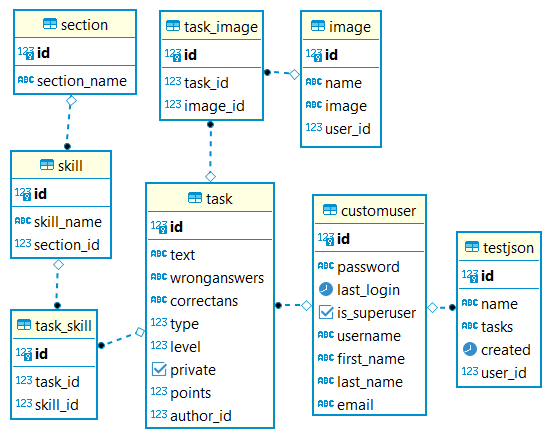
\includegraphics[width=12cm, height=8cm]{gl-relacje.png}
  \caption{Główne tabele}
  \label{relacje}
\end{figure}

\noindent Powyższy rysunek~\ref{relacje} obrazuje głowne tabele znajdujące się w bazie danych naszego projektu. Każda tabela połączona jest z jedną lub wieloma tabelami za pomocą relacji.

Relacjami nazywamy skojarzenia między dwoma typami jednostek. W relacyjnej bazie danych działają one między dwiema tabelami, przy czym jedna tabela posiada klucz obcy klucza podstawowego drugiej tabeli. Dzięki relacjom możemy dzielić i przechowywać dane w różnych tabelach.

W Django możliwe jest użycie trzech najpopularniejszych typów relacji w~bazie danych:

\begin{itemize}
\item Jeden do jednego ang. \emph{One-to-one}
\item Jeden do wielu ang. \emph{One-to-many}
\item Wiele do wielu ang. \emph{Many-to-many}

\end{itemize}


\begin{center}
\subsection{Relacje jeden do jednego}
\end{center}

W relacji jeden do jednego tylko jeden rekord tabeli A (najczęściej klucz podstawowy) może być powiązany z innym rekordem tabeli B mającym taką samą wartość. Przykładem może być uczeń, który posiada tylko jedną szafkę w szkole.
W Django należy użyć typu \texttt{OneToOneField}, aby zdefiniować relację jeden do jednego.
\begin{lstlisting}[
language={Python},
xleftmargin=14pt,
caption={Jeden do jednego Student-School locker}
]
class School_locker(models.Model):
    address = models.CharField(max_length=50)

    def __str__(self):
        return self.address


class Student(models.Model):
    name = models.CharField(max_length=25)
    locker = models.OneToOneField(
        School_locker,
        on_delete=models.CASCADE,
        primary_key=True,
    )

    def __str__(self):
        return self.name
\end{lstlisting}

\begin{center}
\subsection{Relacje jeden do wielu}
\end{center}

Relacja jeden do wielu jest najczęściej używanym typem połączenia i odpowiada sytuacji, gdy pojedynczemu rekordowi z tabeli A jest przyporządkowany jeden lub wiele rekordów z tabeli B, natomiast pojedynczemu rekordowi z tabeli B jest przyporządkowany dokładnie jeden rekord z tabeli A.
Aby zdefiniować relację jeden do wielu w Django, należy użyć \textbf{ForeignKey}. Przykładem mogą być modele \texttt{Section} (dział) oraz \texttt{Skill} (umiejętność) zawarte w projekcie.  \newpage 
\begin{lstlisting}[
language={Python},
xleftmargin=14pt,
caption={Jeden do wielu Section-Skill}
]
class Section(models.Model):
    section_name = models.CharField(max_length=500, unique=True)
	# ...


class Skill(models.Model):
    skill_name = models.CharField(max_length=500, unique=True)
    section = models.ForeignKey(Section, on_delete=models.CASCADE)
	# ...

\end{lstlisting}

\begin{figure}[H]
  \centering
  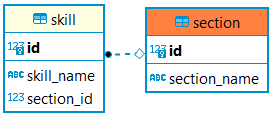
\includegraphics[width=6cm]{skillsec.png}
  \caption{Wiele do jednego Section-Skill}
  \label{obraz-przyklad}
\end{figure}

W modelu Skill zawarty jest klucz obcy modelu Section, co pozwala na przypisanie kilku umiejętności do jednego działu.

\begin{center}
\subsection{Relacje wiele do wielu}
\end{center}
Relacja wiele do wielu występuje w sytuacji, gdy rekordowi tabeli A przyporządkowany jest jeden lub wiele rekordów tabeli B. Sytuacja ta ma miejsce również z~drugiej strony.
Aby zdefiniować relację wiele do wielu w Django, należy użyć \texttt{ManyToManyField}. Za przykład można obrać model \texttt{Task} (zadanie) oraz \texttt{Skill} (umiejętność).
\begin{lstlisting}[
language={Python},
xleftmargin=14pt,
caption={Wiele do wielu Task-Skill}
]
class Skill(models.Model):
    skill_name = models.CharField(max_length=500, unique=True)
    section = models.ForeignKey(Section, on_delete=models.CASCADE)
    	# ...


class Task(models.Model):
    	# ...
    skill = models.ManyToManyField(Skill)
    	# ...
\end{lstlisting}

Sposób w jaki obiekty są ze sobą wiązane za pomocą relacji wiele do wielu znacząco różni się od radzenia sobie z kluczem obcym, ponieważ wymagane jest zapisanie umiejętności w bazie danych, zanim przypisana zostanie do zadania i~odwrotnie. Dzieje się tak, ponieważ \texttt{ManyToManyField} tworzy \textbf{pośrednią tabelę złączeń}, która wiąże model źródłowy z modelem docelowym. Aby stworzyć połączenie między modelami, oba muszą zostać dodane do tego niewidocznego modelu. Dokumentacja \href{https://docs.djangoproject.com/en/4.0/ref/models/fields/#:~:text=If%20you%20don%E2%80%99t%20specify%20an,instance%20like%20a%20normal%20model%3A}{Django} informuje, że:
\begin{quotation}
...nadal istnieje niejawna klasa modelu, której możesz użyć do bezpośredniego dostępu do tabeli utworzonej do przechowywania skojarzenia. Posiada trzy pola do łączenia modeli.

Jeśli model źródłowy i docelowy różnią się, generowane są następujące pola:

\textbf{id}: klucz główny relacji

\textbf{<zawierający\_model>\_id}: model \textbf{id}, który deklaruje \textbf{ManyToManyField}

\textbf{<inny\_model>\_id}: model \textbf{id}, który wskazywany jest przez \textbf{ManyToManyField}
\end{quotation}
Niewidoczny model pośredni stworzony przez Django wymaga pary kluczy. Jest to klucz podstawowy modelu źródłowego oraz klucz modelu docelowego, dlatego oba obiekty muszą istnieć, zanim będą mogły zostać powiązane.

\begin{figure}[H]
  \centering
  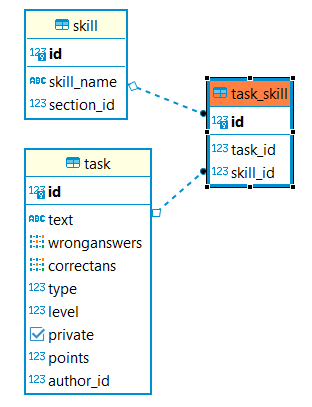
\includegraphics[scale=0.8]{task_skill.png}
  \caption{Wiele do wielu Task-Skill}
  \label{obraz-przyklad}
\end{figure}

W przypadku projektu stworzona została tabela o nazwie \texttt{task\_skill} zawierająca trzy kolumny: \texttt{id}, \texttt{task\_id} oraz \texttt{skill\_id}.

\begin{center}
\subsection{Integralność danych}
\end{center}
Wszystkie relacje tworzą zależności między połączonymi modelami, więc ważne jest, aby określić co dzieje się z drugą stroną, gdy pierwsza zostanie usunięta.
W~tym celu została stworzona opcja \texttt{on\_delete}, której zadaniem jest określać, co należy zrobić z rekordami, których druga strona została usunięta. Opcja ta jest dostępna dla wszystkich trzech relacji i może przyjmować następujące wartości:

\begin{itemize}
\item \texttt{on\_delete=models.CASCADE} - Automatycznie usuwa powiązane rekordy, które były powiązane z daną instancją.
\item \texttt{on\_delete=models.PROTECT} - Zapobiega usunięciu powiązanej instancji.
\item \texttt{on\_delete=models.SET\_NULL} - Przypisuje \texttt{NULL} do powiązanych rekordów, gdy powiązana instancja jest usuwana. Należy pamiętać aby użyć opcji \texttt{null=True} w polu.
\item \texttt{on\_delete=models.SET\_DEFAULT} - Przypisuje wartość domyślną do powiązanych rekordów, gdy powiązana instancja jest usuwana.
\item \texttt{on\_delete=models.SET} - Przypisuje wartość ustawioną przez wywołanie do powiązanych rekordów, gdy powiązana instancja zostanie usunięta.
\item \texttt{on\_delete=models.DO\_NOTHING} - Żadne działanie nie jest podejmowane po usunięciu powiązanych rekordów. Zwykle jest to zła praktyka dotycząca relacyjnych baz danych, ponieważ powstają osierocone rekordy bez wartości.
\end{itemize}
\section{ORM w Django}
Mapowanie obiektowo-relacyjne (ang. \emph{Object-Relational Mapping} -- ORM) -- sposób odwzorowania obiektowej architektury systemu informatycznego na bazę danych (lub inny element systemu) o relacyjnym charakterze. Dzięki ORM możliwe jest pisanie kodu np. w języku Python zamiast SQL. Framework Django wyposażony jest we własny, wbudowany moduł zwany ,,Django ORM'' oraz udostępnia interfejs \texttt{QuerySet}, który umożliwia tworzenie, pobieranie, aktualizowanie i usuwanie obiektów. Są to polecenia, dzięki którym możliwe jest pobieranie informacji z~bazy danych oraz otrzymywanie ich w postaci obiektów. Polecenia te możemy wykonywać z pomocą konsoli po wpisaniu następującej komendy:
\begin{lstlisting}[style=DOS]
>python manage.py shell
\end{lstlisting}
Kolejnym wymogiem jest zaimportowanie modeli, na których chcemy pracować.
\begin{lstlisting}[style=DOS]
>>>from projekt.models import Task, CustomUser, Skill
\end{lstlisting}
W tym momencie mamy możliwość tworzenia, otrzymywania oraz filtrowania obiektów.

\begin{center}
\subsection{Tworzenie obiektu}
\end{center}
\begin{lstlisting}[
style=DOS,
caption={.},
label={taskcreate}
]
>>>user = CustomUser.objects.get(id = 1)
>>>skill = Skill.objects.get(id = 1)
>>>task = Task.objects.create(text = 'zadanie przyklad',
	wrong_answers = [20,12,32], correct_answers = [21],type = 2,
	author = user,level = 1, private = False, points = 2)
>>>task.skill.add(skill)

\end{lstlisting}
W powyższym przykładzie~\ref{taskcreate} należy początkowo pobrać z bazy obiekt użytkownika oraz wybraną umiejętność. Następnym krokiem jest utworzenie obiektu \texttt{Task} przy pomocy metody \texttt{create} i po wprowadzeniu odpowiednich danych. Na końcu należy przypisać obiekt \texttt{skill} do pola \texttt{task.skill}. Poniżej znajduje się skrypt SQL~\ref{taskcreatesql} wykonany przez Django.
\begin{lstlisting}[
style=DOS,
caption={.},
label={taskcreatesql}]
SELECT "customuser"."id",
       "customuser"."password",
	  ...
  FROM "customuser"
 WHERE "customuser"."id" = 1

SELECT "skill"."id",
       "skill"."skill_name",
       "skill"."section_id"
  FROM "skill"
 WHERE "skill"."id" = 1

INSERT INTO "task" ("text", "wrong_answers",
		"correct_answers", "type", "author_id",
		"level", "private", "points")
VALUES ('zadanie przyklad', ARRAY['20','12','32']::varchar(200)[],
	ARRAY['21']::varchar(200)[], 2, 1, 1, false, 2) 
	RETURNING "task"."id"
\end{lstlisting}

\begin{center}
\subsection{Pobieranie obiektu}
\end{center}
Pobieranie danych z bazy może być wykonane na wiele sposobów. Oto kilka metod:

\begin{itemize}
\item \texttt{all()} - zwraca wszystkie rekordy danego modelu
\item \texttt{get()} - zwraca tylko jeden rekord spełniający warunek w \texttt{get()}
\item \texttt{filter()} - zwraca rekordy spełniające warunek w \texttt{filter()}
\item \texttt{reverse()} - obiekty zwracane będą w odwrotnej kolejności
\item \texttt{distinct()} - zwraca tylko unikalne obiekty bez duplikatów
\end{itemize}

Pobieranie obiektów z bazy danych czasem może trwać długo, dlatego istotne jest to, aby wykonywane skrypty działały w sposób optymalny. 

Ważnym jest, że zapytania wykonują się dopiero w momencie odniesienia do danych. Jeśli po raz kolejny wykonamy to samo zapytanie, czas odpowiedzi będzie krótszy, ponieważ wynik zapytania zapisany będzie w cache.
\begin{lstlisting}[
style=DOS,
caption={.},
label={taskall}]
>>>tasks = Task.objects.all()
>>>list(tasks)
>>>tasks[0]
\end{lstlisting}
W powyższym przykładzie~\ref{taskall} zapytanie zostało wykonane dopiero w drugiej linii. Element listy \texttt{tasks[0]} został zapamiętany, więc zapytanie nie zostało ponownie wywołane.

Zdarza się, że podczas pozyskiwania danych z bazy zostają pobrane całe obiekty, mimo że wykorzystywane jest jedynie kilka parametrów. Takie działanie może znacząco wpłynąć na czas wykonania, dlatego warto skorzystać z \texttt{values} (wynik w formie słownika), lub \texttt{values\_list} (wynik w formie listy)
\begin{lstlisting}[style=DOS]
>>> Task.objects.all()
SELECT "task"."id",
       "task"."text",
       "task"."wrong_answers",
       "task"."correct_answers",
       "task"."type",
       "task"."author_id",
       "task"."level",
       "task"."private",
       "task"."points"
  FROM "task"

>>> Task.objects.values("text")
SELECT "task"."text"
  FROM "task"
\end{lstlisting}
Przechodząc po liście obiektów tylko raz, można wykorzystać do tego iterator, który podczas iteracji odwoływać się będzie do kolejnych elementów. W~ten sposób unikniemy niepotrzebnego ładowania całego zapytania. Poniższy przykład~\ref{fastquery} ukazuje o wiele szybsze działanie polecenia przy użyciu iteratora.
\begin{lstlisting}[
style=DOS,
caption={.},
label={fastquery}]
>>> for task in Task.objects.all():
...     text = task.text
SELECT "task"."id",
	...
  FROM "task"
Execution time: 0.011384s [Database: default]
>>> for task in Task.objects.all().iterator():
...     text = task.text
DECLARE "_django_curs_140417171636352_sync_8" NO SCROLL
CURSOR WITH HOLD
   FOR SELECT "task"."id",
		...
  FROM "task"
Execution time: 0.002761s [Database: default]
\end{lstlisting}

Funkcja \texttt{select\_related} podczas wykonywania zapytania podąża za relacjami klucza obcego, pobierając odpowiednie dane obiektu powiązanego relacją.
Funkcja ta, w przeciwieństwie do wykonywania wielu zapytań, pozwala na stworzenie jednego, złożonego, w którym użycie klucza obcego nie będzie skutkowało wykonaniem kolejnego zapytania. Przykładem będzie sytuacja, w~której dla dziesięciu zadań posiadających umiejętność o \texttt{id} równym 6, chcemy wypisać ich autorów.
\begin{lstlisting}[
style=DOS,
caption={.},
label={execution}]
>>> id_of_authors = []
>>> e = Task.objects.filter(skill=6)[:10]
>>> exec("for task in e: text = print(task.author.id)")
SELECT "task"."id",
	...
  FROM "task"
 INNER JOIN "task_skill"
    ON ("task"."id" = "task_skill"."task_id")
 WHERE "task_skill"."skill_id" = 6
 LIMIT 10
Execution time: 0.001817s [Database: default]
SELECT "customuser"."id",
	...
 WHERE "customuser"."id" = 2
 LIMIT 21
Execution time: 0.001256s [Database: default]
Execution time: 0.001192s [Database: default]
Execution time: 0.001339s [Database: default]
Execution time: 0.001212s [Database: default]
Execution time: 0.001298s [Database: default]
Execution time: 0.001349s [Database: default]
Execution time: 0.001313s [Database: default]
Execution time: 0.001406s [Database: default]
Execution time: 0.001275s [Database: default]
Execution time: 0.001305s [Database: default]
>>> print(id_of_authors)
[2, 4, 4, 3, 4, 2, 1, 3, 4, 3]
\end{lstlisting}
Powyższy kod~\ref{execution} bez użycia \texttt{select\_related()} wykona aż $11$ zapytań do bazy. Jedno zwracające zadania, a każde kolejne o autora w pętli. Łączny czas wykonywanie wynosi $0.012945$s. Poniżej znajduje się kod~\ref{selectrelated} wykorzystujący \texttt{select\_related()}, który dokona tylko jednego zapytania, a czas wynosić będzie $0.002796$s.
\begin{lstlisting}[
style=DOS,
caption={.},
label={selectrelated}]
>>> id_of_authors = []
>>> e = Task.objects.select_related('author').filter(skill=6)[:10]
>>> exec("for task in e: text = print(task.author.id)")
SELECT "task"."id",
	...
       "customuser"."id",
	...
  FROM "task"
 INNER JOIN "task_skill"
    ON ("task"."id" = "task_skill"."task_id")
 INNER JOIN "customuser"
    ON ("task"."author_id" =
Execution time: 0.002796s [Database: default]
>>> print(id_of_authors)
[2, 4, 4, 3, 4, 2, 1, 3, 4, 3]
\end{lstlisting}

\begin{center}
\subsection{Aktualizacja obiektu}
\end{center}

Metoda \texttt{update()} wykonuje zapytanie aktualizujące SQL dla określonych pól i zwraca liczbę dopasowanych wierszy. Na przykład, aby zmienić typ wszystkich zadań o punktacji równej $4$ potrzebne jest polecenie:\\

\begin{lstlisting}[style=DOS]
>>> Task.objects.filter(points = 4).update(type = 1)
UPDATE "authentication_task"
   SET "type" = 1
 WHERE "authentication_task"."points" = 4
Execution time: 0.170321s [Database: default]
\end{lstlisting}

\begin{center}
\subsection{Usuwanie obiektu}
\end{center}
Metoda \texttt{delete()} wykonuje zapytanie SQL usuwające dla wszystkich wierszy w QuerySet.
\begin{lstlisting}[style=DOS]
>>> Task.objects.filter(points = 1).delete()
\end{lstlisting}

\begin{center}
\section{Wyzwalacze Django-PostgreSQL}
\end{center}
Wyzwalacze mogą rozwiązywać wiele różnych problemów na poziomie bazy danych lepiej niż na poziomie aplikacji Django. Dzięki wyzwalaczom możliwa jest np.:
\begin{itemize}
\item ochrona przez usuwaniem oraz zmienianiem wierszy lub kolumn
\item śledzenie zmian w modelach lub kolumnach
\item synchronizacja pól z innymi polami.
\end{itemize}
Aby używać wyzwalaczy bazy PostgreSQL w Django z pomocą przychodzi dodatek \texttt{django-pgtrigger}.
\begin{lstlisting}[style=DOS]
>pip install django-pgtrigger
\end{lstlisting}
Wykonując powyższe polecenie oraz dodając \texttt{pgtrigger} do \textbf{INSTALLED\_APPS} można rozpocząć współpracę z \texttt{django-pgtrigger}.
\begin{center}
\subsection{Ochrona przed usunięciem modelu}
\end{center}

Definicja pgtrigger.Protect wywołuje ochronę przed wykonaniem wybranej operacji.
\begin{lstlisting}[
language={Python},
xleftmargin=5pt,
xrightmargin=5pt,
caption={Fragment pliku \texttt{models.py}}
]
import pgtrigger
@pgtrigger.register(
    pgtrigger.Protect(
        name="delete_protect", operation=pgtrigger.Delete)
)
class Section(models.Model):
   ...
\end{lstlisting}
\begin{lstlisting}[style=DOS]
>>> section = Section.objects.get(id=3)
>>> section.delete()
django.db.utils.InternalError: pgtrigger: 
 Cannot delete rows from section table
CONTEXT:  
 PL/pgSQL function pgtrigger_protect_deletes_f1129() line 14 at RAISE
\end{lstlisting}
Chcąc usunąć dział o \texttt{id} równym 3 otrzymujemy błąd informujący o tym, że operacja ta nie jest możliwa. Takie działanie daje nam pewność, że działy lub umiejętności nie zostaną usunięte.
\begin{center}
\subsection{Możliwość wyłącznie tworzenia lub odczytu}
\end{center}

Wyzwalacz \texttt{pgtrigger.Protect} oferuję nie tylko ochronę przed usunięciem modelu. Kolejną przydatną opcją jest ochrona przez aktualizowaniem danych modelu.
\begin{lstlisting}[
language={Python},
label={pgtrigg},
xleftmargin=5pt,
xrightmargin=5pt,
caption={Fragment pliku \texttt{models.py}}
]
@pgtrigger.register(
    pgtrigger.Protect(
        name="delete_update_protect",
        operation=(pgtrigger.Update | pgtrigger.Delete)
    )
)
class Task(models.Model):
   ...
\end{lstlisting}
Powyższy kod~\ref{pgtrigg} ukazuję ochronę modelu, dającą możliwość jedynie tworzenia nowego zadania w bazie. Próba zmiany jego wartości lub usunięcia skutkować będzie błędem. Możliwa jest również ochrona poszczególnego pola modelu.
Jeżeli chcemy, aby użytkownik nie mógł zmieniać typu lub poziomu zadania, należy użyć:

\begin{lstlisting}[
language={Python},
xleftmargin=5pt,
xrightmargin=5pt,
caption={Fragment pliku \texttt{models.py}}
]
@pgtrigger.register(
    pgtrigger.Protect(
        operation=pgtrigger.Update,
        name="type_level_protect",
        condition=(
            pgtrigger.Q(old__type__df=pgtrigger.F("new__type")),
            pgtrigger.Q(old__level__df=pgtrigger.F("new__level"))
        )
    )
)
class Task(models.Model):
   ...
\end{lstlisting}

\begin{center}
\subsection{Miękkie usuwanie}
\end{center}
Zdarza się, że użytkownik usunie utworzony przez siebie sprawdzian, lecz po pewnym czasie chce go odzyskac. Można użyć wtedy \texttt{pgtrigger.SoftDelete}, który zapobiegnie całkowitemu usunięciu obiektu, poprzez zmianę wartości pola obiektu.
\begin{lstlisting}[
language={Python},
xleftmargin=5pt,
xrightmargin=5pt,
caption={Fragment pliku \texttt{models.py}}
]
@pgtrigger.register(
    pgtrigger.SoftDelete(
        name="soft_del",
        field="is_active", value=False)
)
class Test(models.Model):
    is_active = models.BooleanField(default=True)
    ... 
\end{lstlisting}
Gdy użytkownik usunie sprawdzian, pole \texttt{is\_active} zmieni swoją wartość na \texttt{False} i nie będzie juz wyświetlane na jego liście. Jeśli jednak będzie on chciał owy sprawdzian odzyskać, musi zrobić to z listy usuniętych sprawdzianów lub przez inne przeznaczone do tego rozwiązanie.
\begin{center}
\subsection{Śledzenie zmian}
\end{center}

Jeżeli potrzebna jest możliwość śledzenia zmian w modelach użyteczne może okazac się \texttt{django-pghistory}, które zapewnia automatyczne i konfigurowalne śledzenie historii dla modeli Django przy użyciu wyzwalaczy. Aby używać \texttt{django-pghistory} potrzebne również będzie zainstalowanie aplikacji \texttt{django-pgconnection} oraz odpowiednie skonfigurowanie pliku settings.py. Po instalacji należy wykonać migrację.
\begin{lstlisting}[
language={Python},
xleftmargin=5pt,
xrightmargin=5pt,
caption={Fragment pliku \texttt{settings.py}}
]
DATABASES = pgconnection.configure(
    {
        "default": {...}
    }
)

\end{lstlisting}
Przykładem użycia \texttt{django-pghistory} może być potrzeba zbierania informacji na temat utworzenia nowych zadań matematycznych.
\begin{lstlisting}[
language={Python},
label={pgtrigger},
xleftmargin=5pt,
xrightmargin=5pt,
caption={Fragment pliku \texttt{settings.py}}
]
@pghistory.track(
    pghistory.AfterInsert("create")
)

class Task(models.Model):
	...
\end{lstlisting}
Powyższy kod~\ref{pgtrigger} pozwala na zapisywanie informacji dotyczących tworzonych zadań przez użytkowników. W tym celu Django stworzył nową tabele \texttt{taskevent}, gdzie zapisywane są wszelkie dane.
Istnieje wiele innych zastosowań \texttt{django-pghistory}. Aby poznać wszystkie z nich, warto zapoznać się z~dokumentacją.

\section{Podsumowanie}
W tym rozdziale zawarte zostały informacje na temat współpracy frameworka Django z bazą danych PostgreSQL. Treści te pokazują w jaki sposób poprawnie łączyć się z bazą, tworzyć modele oraz wykorzystywać relację na przykładzie projektu Generatora Sprawdzianów. Opisane zostało również, jak w optymalny sposób odpytywać bazę danych oraz wykorzystywać przydatne pakiety mające na celu pomoc we współpracy z PostgreSQL.

\chapter {React jako narzędzie do tworzenia interfejsu użytkownika}

\section{Czym jest React?}
{
React jest javascriptową biblioteką typu open-source\footnote{open source - rodzaj oprogramowania oparty na licencji przyznającej użytkownikom prawo do badania, zmiany i rozpowszechniania oprogramowania ~\cite{opensourcewiki}} używaną do tworzenia interfejsów użytkownika aplikacji internetowych. Jego oryginalnym autorem jest programista firmy Facebook - Jordan Walke. Pierwszy, bardzo wczesny prototyp Reacta - FaxJS powstał już w 2011 roku i został wykorzystany do zaimplementowania funkcji "Szukaj" na platformie Facebook. Niewiele później, aby móc łatwiej obsługiwać Facebook Ads, Jordan rozwinął prototyp i stworzył React. Po nabyciu przez Facebooka Instagrama w 2012 roku, Instagram wyrażał chęć wdrożenia nowej technologii na swoją platformę, co powodowało nacisk na odłączenie Reacta od Facebooka i przejście na licencję open-source. W 2013 roku biblioteka przeszła na licencję open source ~\cite{reactstory}. 
\newline
Od tamtego momentu React cały czas prężnie się rozwija, pozostaje jednym z~ najpopularniejszych narzędzi do tworzenia interfejsów graficznych, używany jest nie tylko przez ogromne firmy takie jak Uber, Netflix, Airbnb, Amazon, Twitter oraz wiele innych, ale również przez zwykłych użytkowników. Popularność Reacta nie przestaje rosnąć, w styczniu 2021 roku biblioteka została pobrana ponad 10 milionów razy - zdecydowanie wyróżniając się na tle podobnych narzędzi przeznaczonych do tworzenia interfejsów użytkownika.
%###############################################################

\begin{figure}
\centering
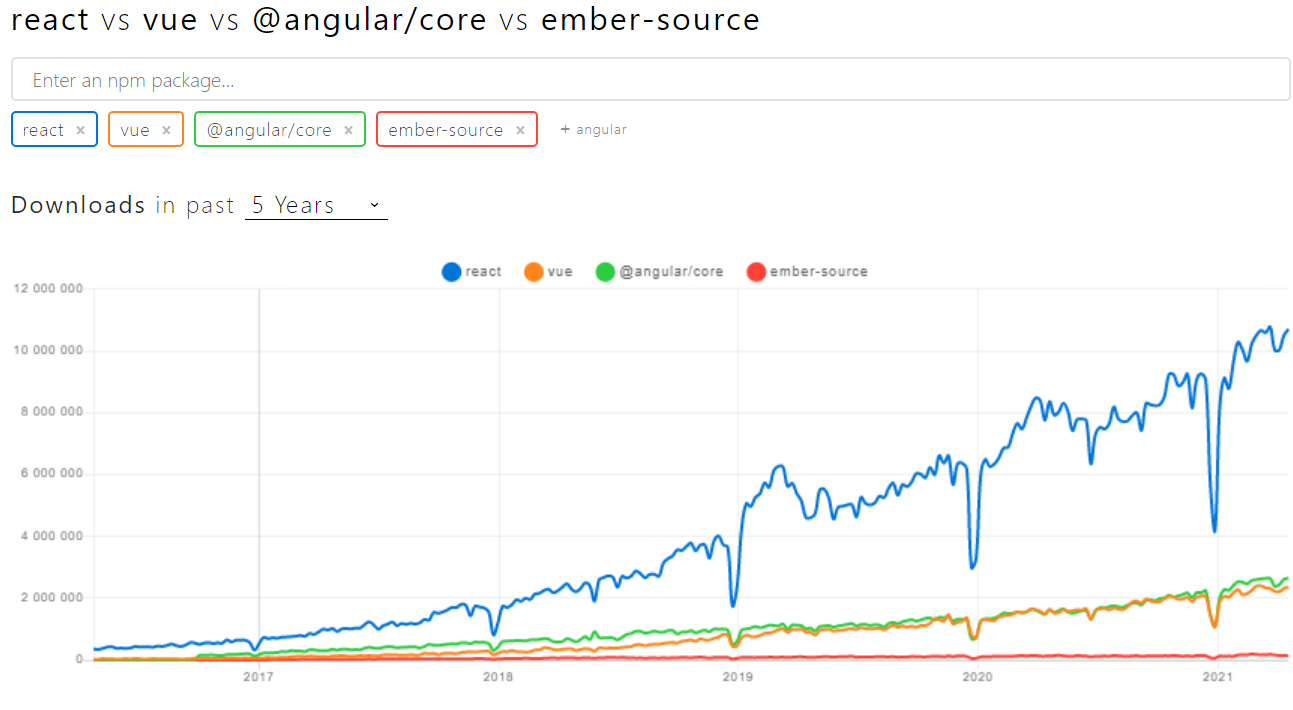
\includegraphics[width=14cm]{statystyki react vue angular.png}
\caption{npm trends, statystyki dotyczące ilości pobrań popularnych narzędzi do tworzenia interfejsów}
\label{statystyki react vue angular.png}
\end{figure}

}

\section{Dlaczego warto korzystać z Reacta?}{
React posiada wiele zalet, które sprawiły, że został użyty w projekcie. Relatywnie niska bariera wejścia, dzięki której nauka powinna być w miarę prosta dla osób mających wcześniejszą styczność z programowaniem. Łatwość testowania oraz debugowania - w tym celu bardzo przydatne jest narzędzie React Developer Tools, którego możemy używać z poziomu przeglądarki internetowej. React Developer Tools jest dostępne w postaci rozszerzenia, po którego zainstalowaniu ujrzymy dwie zakładki, zakładkę Components oraz zakładkę Profiler. W zakładce Components możemy obserwować hierarchię wszystkich komponentów naszej aplikacji, dowolnego komponentu oraz to jak zmienia się on w czasie. Druga zakładka Profiler pozwala nam sprawdzić wydajność naszej aplikacji. Domyślnie React pokazuje programiście wiele użytecznych, dobrze opisanych komentarzy oraz ostrzeżeń usprawniających pracę, są one dostępne, kiedy aplikacja znajduje się w fazie developerskiej. Wszystko to sprawia, że aplikacja w fazie developerskiej działa wolniej. Przejście do fazy produkcyjnej usuwa większość komentarzy, ostrzeżeń oraz możliwość sprawdzania każdego komponentu i dowolnej informacji o nim przy pomocy React Developer Tools, ale za to znacząco przyspiesza wydajność aplikacji.
Właśnie z tych powodów tryb developerski stosujemy w czasie budowania aplikacji, a trybu produkcyjnego w ostatecznej wersji produktu, która ma trafić do użytkownika.




\begin{figure}[H]
\centering
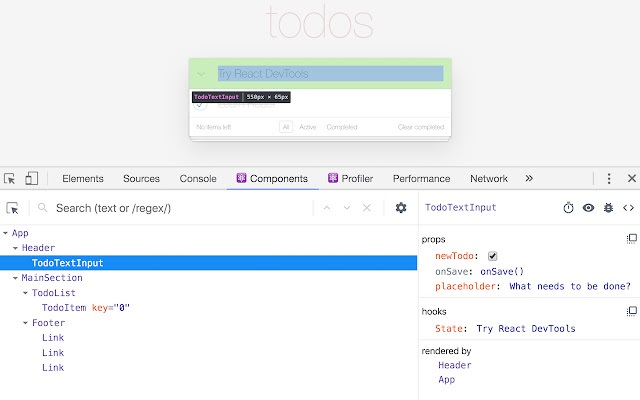
\includegraphics[width=13cm]{react dev example.jpg}
\caption{React Developer Tools - obraz poglądowy
\newline
Źródło: \url{https://lh3.googleusercontent.com/XWuZGqIrIsaoKHUqqQ2rs_GhS5JaH1p5pPBIUpj22mjNRNdR3Ana8FKz4B7JwsA6HIFVXGuU7pa4ELiW6iUNhs0Iyg=w640-h400-e365-rj-sc0x00ffffff}
}
\label{react dev example.jpg}
\end{figure}

React posiada obszerną, bardzo dobrze napisaną dokumentację wraz z samouczkiem 
~\cite{reactjs} dostępną w wielu językach, między innymi w języku Polskim.
Kolejnym z plusów jest budowa komponentów, interfejs zbudowany w Reaccie jest stworzony z mniejszych komponentów, które łączą w sobie wygląd wraz z logiką odpowiedzialną za ich zachowanie, co pomaga w zorganizowaniu pracy, dodatkową pomocą jest JSX - rozszerzenie składni pozwalające na używanie znaczników HTML razem z językiem Javascript.
Ogromna popularność Reacta przekłada się również na mnogość dostępnych samouczków i innych materiałów pozwalających lepiej zrozumieć tę bibliotekę. Dodatkowo w poszukiwaniu odpowiedzi na nurtujące nas pytania możemy zajrzeć do społeczności programistów React takich jak dev.to, hashnode, lub najpopularniejszy z nich pod względem obserwujących użytkowników (aktualnie jest ich ponad ćwierć miliona) - Reddit.
}




\section{Npm}{

Npm (pierwotnie skrót od Node Package Manager) jest to manager pakietów języka Javascript. Pierwsze wydanie npm miało miejsce już w 2010 roku~\cite{npmwiki}.
Npm jest domyślnym managerem pakietów środowiska Node.js, npm jest instalowane razem z Node.js. Najważniejszym aspektem npm jest ogromna baza pakietów, bibliotek o 
niezwykle szerokim wachlarzu zastosowań. Interesujące nas rozszerzenie możemy zainstalować przy pomocy komendy
\newline
\textit{npm install nazwapakietu}
\newline
Kiedy nad projektem pracuje wiele osób, ilość używanych bibliotek może rozrastać się dużo szybciej wraz z szukaniem nowych rozwiązań do pojawiających się problemów.
Potrzeba wpisywania nazwy każdego pakietu oraz instalowania go osobno mogłaby być męcząca, dlatego npm śledzi wszystkie używane w danym projekcie pakiety w jsonowym pliku
packages. Aby zainstalować wszystkie pakiety zarejestrowane przez plik packages należy użyć komendy
\newline
\textit{npm update}
\newline





}



\section{Pojęcia Reacta}


% #$#$#$#$#$#$#$#$#$#$#$##$#$#$#$#$#$#$#$#$#$#$##$#$#$#$#$#$#$#$#$#$#$##$#$#$#$#$#$#$#$#$#$#$#

\subsection{JSX}

{
JSX, czyli Javascript XML jest rozszerzeniem składni języka Javascript, które pozwala na używanie znaczników HTML razem z językiem Javascript. Jest to niezwykle przydatne narzędzie, które ułatwia nam na operowanie danymi przetwarzanymi w kodzie Javascriptowym oraz ułatwia ich wyświetlanie przy pomocy znaczników HTML. JSX możemy wykorzystać w wielu celach.



\begin{lstlisting}[
caption={Fragment pliku MaterialUiUserExams.js, przykładowe użycie JSX}
]
<ListItemText>
	primary={<h3>{section.Section}</h3>}
	secondary={"Dostępnych zadań: " + section.sectionTaskCount}
</ListItemText>
\end{lstlisting}



Jedną z zalet JSX jest łatwość otrzymania wartości zmiennej używanej w kodzie javascriptowym. W powyższym przykładzie wykorzystujemy to, aby otrzymać nazwę każdego działu, który następnie wyświetlamy użytkownikowi.
JSX jest w stanie obsłużyć dowolne, prawidłowe wyrażenie w języku Javascript, które zostało zamknięte wewnątrz nawiasów klamrowych. Dzięki czemu możemy nie tylko uzyskać wartości zmiennych, ale również je modyfikować oraz wywoływać funkcje javascriptowe, jeśli tego potrzebujemy.



\begin{lstlisting}[
caption={Wywołanie funkcji map wewnątrz elementu <List>}
]
<List>
 {sections.map((section) => {
                     
	  return (
	 <>
	 <ListItem
	 button onClick={this.hideSection(section)}>

		 <ListItemText>
		 primary={<h3>{section.Section}</h3>}
		 secondary={"Dostępnych zadań: " + section.sectionTaskCount}
		 </ListItemText>
		 {(this.state.hiddenSections.indexOf(section.id) !== -1)
		 ? <ExpandLess /> : <ExpandMore />}
	 </ListItem>

		 <Collapse in={(this.state.hiddenSections
			.includes(section.id))} 
		timeout="auto" unmountOnExit>
			 <List component="div" disablePadding>
			 <ListItem button
			 key={section.id}
			 onClick={this.handleToggleAll(section)}>
			 <ListItemIcon>
			 	<Checkbox
			 	edge="start"
			 	checked={this.state.
				fullyChecked.indexOf(section.id) !== -1}
				 tabIndex={-1}/>
			 </ListItemIcon>
			 <ListItemText 
			 primary={<b>Zaznacz wszystkie</b>}  />
	 </ListItem>
...
</List>
\end{lstlisting}



Po kompilacji wyrażenia JSX stają się wywołaniami funkcji w języku Javascript, oznacza to, że możliwe jest używanie wyrażeń w JSX wewnątrz instrukcji warunkowych, pętli, przypisywanie je do zmiennych, używanie jako argumentów oraz zwracanie z funkcji.
Oczywiście, jeśli ktoś nie chce korzystać z JSX, może tego nie robić. Możliwe jest stworzenie wszystkich komponentów w czystym Javascripcie, natomiast JSX jest narzędziem bardzo wygodnym, mocno usprawniającym pracę z Reactem, dlatego jest zdecydowanie zalecanym rozwiązaniem.

}

\subsection{Komponenty}
{
Interfejs w React składa się z komponentów. Komponenty są jak funkcje javascriptowe, które przyjmują pewne wartości na wejściu, a następnie zwracają elementy reactowe, które opisują, co ma pojawić się na ekranie.
Wyróżniamy dwa typy komponentów - komponenty klasowe oraz komponenty funkcyjne.


\begin{lstlisting}[
caption={Przykład komponentu klasowego}
]
class ClassComponent extends Component{
  render(){
    return <h2>Przykład komponentu klasowego</h2>
  }
}

\end{lstlisting}


\begin{lstlisting}[
caption={Przykład komponentu funkcyjnego}
]
function FunctionComponent(props){
  return <h2>Przykład komponentu funkcyjnego</h2>
}

\end{lstlisting}

Jedną z zasad obowiązujących podczas budowy komponentów, zarówno funkcyjnych jak i klasowych pozostaje nienaruszalność właściwości    (ang. props) przekazywanych podczas deklaracji funkcji, dane, które mają zmieniać się dynamiczne powinny być przechowywane w stanach.
Obecnie podstawową różnicą pozostaje składnia, w przeszłości komponenty funkcyjne nie posiadały stanów ani metod pozwalających na uruchamianie kodu w odpowiednich momentach, z tych powodów komponentów funkcyjnych używano tylko do budowy komponentów, które nie musiały być dynamiczne. Zmieniło się to wraz z wprowadzeniem Hooków.
Warto również wiedzieć, że komponenty mogą odwoływać się do innych komponentów, co promuje pisanie ich z myślą o~ możliwości wielokrotnego wykorzystania. Możemy to wykorzystać na przykład tworząc komponent ekranu ładowania, następnie możemy go użyć w innych komponentach, renderując go wtedy, gdy użytkownik będzie oczekiwał na odpowiedź od serwera.
}

\subsection{Stan i cykl życia}{

Stan zawiera dane związane z danym komponentem, które mogą ulegać zmianie. Stan powinien być obiektem javascriptowym, aby go zmodyfikować należy wywołać metodę setState. Dodatkowo, komponenty posiadają metody cyklu życia, które są odpowiedzialne za uruchamianie kodu w odpowiednich momentach.
\newline
Cykl życia komponentu możemy podzielić na 3 etapy:

\begin{itemize}
\item Montowanie (ang. Mounting), czyli pierwsze stworzenie instancji komponentu i włożenie go do drzewa DOM
\item Aktualizacja, czyli zmiany we właściwościach lub stanie komponentu
\item Odmontowanie (ang. Unmounting), czyli usunięcie komponentu z drzewa DOM
\end{itemize}
\begin{figure}[H]
\centering
\includegraphics[width=13cm]{diagram metod cyklu życia.png}
\caption{Diagram metod cyklu życia
\newline
Źródło: \url{https://projects.wojtekmaj.pl/react-lifecycle-methods-diagram/}
}
\label{metody cyklu zycia}
\end{figure}
Każdy cykl wywołuje inny zestaw metod, najważniejszymi metodami wywoływanymi w czasie montowania są constructor - odpowiedzialny za inicjalizację stanu lokalnego oraz związanie(ang. bind) metody obsługi zdarzeń, render oraz componentDidMount - ta metoda jest odpowiednim miejscem do wysłania zapytania, jeśli potrzebujemy pobrać dane z zewnątrz.
W czasie aktualizacji wywołana zostaje analogiczna metoda - componentDidUpdate, a w czasie Odmontowania wywołana zostaje metoda componentWillUnmount - powinniśmy z niej korzystać głównie w celach posprzątania np. wyzerowanie liczników.
\newline
\newline
Stan może przyjąć dowolną wartość, true, false, null, może być liczbą, ciągiem znaków (string) lub tablicą.

\begin{lstlisting}[
caption={Przykład komponentu klasowego korzystającego ze stanów}
]
  class UserExams extends Component {
    constructor(props) {
      super(props);
      this.state = {
        exams: null,
        open: false,
        listExpand:{},
        generatedId: null,
        generatedName: null,
        sections: null,
        groups: null,
        ileotw: '',
        ilezamk: '',
        level: '',
        skills: '', 
        groups: '',
      }
    }
  }

\end{lstlisting}

}


\subsection{Renderowanie warunkowe}

Renderowanie warunkowe umożliwia wyświetlanie elementów na podstawie stanu danej aplikacji. Oznacza to, że jesteśmy w stanie uzależnić interfejs (to, co widzi użytkownik) od wartości zwracanej przez zastosowaną przez nas instrukcje warunkową.
Do renderowania warunkowego możemy użyć klasycznej instrukcji if,

\begin{lstlisting}[
caption={Renderowanie warunkowe przy pomocy instrukcji if}
]
      if (!exams ) {
        return (
          <Loading  message={"Ładowanie kolekcji sprawdzianów"} >
	</Loading>
        );
      }

\end{lstlisting}

operatora warunkowego, często stosowanego jako krótsza wersja instrukcji if,

\begin{lstlisting}[
caption={Renderowanie przy pomocy operatora warunkowego}
]
{editView == "email" ?
	(
		<h1>Widok, który zobaczy użytkownik,
		jeśli warunek zostanie spełniony </h1>
	):
	(
		<h1>Widok, który zobaczy użytkownik
		 jeśli warunek nie zostanie spełniony</h1>
	)


\end{lstlisting}

jak i operatora logicznego \&\&.

\begin{lstlisting}[
caption={Renderowanie warunkowe przy pomocy operatora logicznego \&\&}
]
{
	isSubmitting &&  <LoadingScreenB></LoadingScreenB>
}  



\end{lstlisting}




\subsection{Hooki}
Hooki zostały wprowadzone w wersji 16.8. Pozwalają używać stanów oraz innych funkcjonalności Reacta w komponentach funkcyjnych.
\newline
Jak podają developerzy, głównymi powodami, dla których wprowadzili hooki było to, że:

\begin{itemize}
\item Współdzielenie logiki związanej ze stanem pomiędzy komponentami jest trudne
\item Wraz ze wzrostem złożoności komponentów stają się one zbyt trudne do zrozumienia
\item Klasy są mylące zarówno dla ludzi jak i maszyn
\end{itemize}

Jeśli chcemy skorzystać ze stanu w komponencie funkcyjnym, należy użyć hooka stanu.


\begin{lstlisting}[
caption={Wywołanie hooka stanu}
]
const [editView, setEditView] = React.useState("email");


\end{lstlisting}

Powyższy przykład pokazuje, jak użyć hooka stanu, gdzie editView jest nazwą stanu, a email jest jego wartością początkową. W przypadku potrzeby zaktualizowania wartości należy 
wywołać funkcję setEditView.


\begin{lstlisting}[
caption={Zmiana stanu przy pomocy funkcji setEditView}
]
<Button variant="contained" 
color="primary" 
onClick={(e)=>setEditView("name")}  >
	Zmień nazwę użytkownika
</Button>


\end{lstlisting}

Jeśli chcemy dokonać operacji w określonym cyklu życia komponentu, należy użyć hooka useEffect. Możemy o nim myśleć jak o połączeniu metod componentDidMount, componentDidUpdate oraz componentWillUnmount w jedną.


\begin{lstlisting}[
caption={Przykładowe użycie hooka useEffect}
]
  useEffect(() => {
    const fetchSections = () => {
      console.log("useeffect");
      axiosInstanceNoAuth
        .get("/user/sections2/")
        .then((response) => {
          const parsed = response.data.map((section) => {
            section.skill = section.skilll;
            return section;
          });
          setSections(parsed);
        })
        .catch((error) => {
          setSections(false);
        });
    };
    fetchSections();
  }


\end{lstlisting}

\subsection{Obsługa zdarzeń}
{
Kolejnym pojęciem często używanym w budowaniu interfejsów są zdarzenia. Zdarzenia określają zajście pewnej czynności, którą nasz interfejs jest w stanie wyłapać i następnie obsłużyć.
Przykładowymi zdarzeniami mogą być onClick - w przypadku kliknięcia myszką, onChange - w przypadku modyfikacji elementu lub onSubmit - w przypadku przesłania formularza.
W odróżnieniu od np. HTMLa w React zdarzenia zapisujemy tzw. camelCasem. \footnote{camelCase jest konwencją, w której w nazwach kolejne wyrazy zapisujemy łącznie, a każdy kolejny(nie licząc pierwszego) rozpoczynamy wielką literą}
Instrukcje obsługi zdarzenia są przekazywane jako funkcje.


\begin{lstlisting}[
caption={Przykładowa obsługa zdarzenia onClick}
]
<BootstrapTooltip title="Skopiuj sprawdzian">
	<IconButton  onClick={() => 
	{this.createExamCopy(exam);}}>
		<FileCopyIcon />
	</IconButton>
</BootstrapTooltip>


\end{lstlisting}

}
Powyższy przykład pokazuje jeden ze sposobów obsługi zdarzeń wykorzystywanych w aplikacji Gen-mat. Kliknięcie przycisku IconButton powoduje wywołanie funkcji createExamCopy, która jest odpowiedzialna za utworzenie kopii sprawdzianu.
Innym sposobem na przekazanie instrukcji obsługi zdarzenia jest napisanie funkcji obsługi, następnie jej związanie (ang. bind) i wywołanie jej przy pomocy {\it this}.


\begin{lstlisting}[
caption={Związanie}
]
this.hideSection = this.hideSection.bind(this);


\end{lstlisting}

\begin{lstlisting}[
caption={Wywołanie obsługi zdarzenia po związaniu}
]
<ListItem
button 
onClick={this.hideSection(section)}>


\end{lstlisting}



\section{Tworzenie formularzy oraz wymiana danych z serwerem} \mbox{}\\
%\bigbreak
Jedną z podstawowych rzeczy, które musi zrobić prawie każdy interfejs w dzisiejszych aplikacjach internetowych jest obsługa formularzy oraz wymiana danych między serwerem, aplikacją oraz użytkownikiem. Interfejs projektu Gen-mat w tym celu używa głównie trzech bibliotek:\newpage

\begin{itemize}
\item Axios
\item Formik
\item Yup
\end{itemize}

\subsection{Axios}
Axios~\cite{axios} jest Klientem HTTP dla node.js oraz przeglądarki, opartym na javascriptowym obiekcie Promise, który służy do obsługi operacji asynchronicznych.

\begin{figure}[H]
\centering
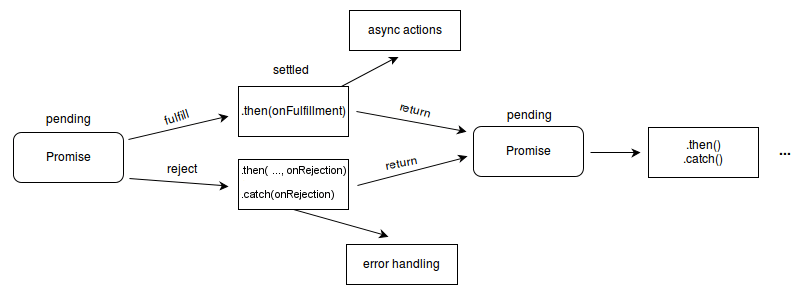
\includegraphics[width=13cm]{promises.png}
\caption{Jak działa Promise?
\newline
Źródło: \url{https://developer.mozilla.org/en-US/docs/Web/JavaScript/Reference/Global_Objects/Promise/promises.png}
}
\label{react dev example.jpg}
\end{figure}

Dzięki Axios możemy tworzyć requesty - żądania HTTP, które są podstawową formą komunikacji z serwerem. HTTP opisuje formę żądania klienta oraz formę odpowiedzi na żądanie ze strony serwera. Do najważniejszych metod HTTP, na których się skupimy, należą:

\begin{itemize}
\item GET - metoda wysyłająca żądanie otrzymania danych, powinna być ograniczona jedynie do pobierania danych, nie powinna ich przesyłać
\item PUT - metoda używana w celu przesłania danych między klientem  oraz serwerem w celu aktualizacji wybranego zasobu
\item POST - metoda używana w celu przesłania danych między klientem  oraz serwerem
\item DELETE - żądanie usunięcia danych
\end{itemize}

Axios pozwala na tworzenie instancji z własną konfiguracją, która będzie stosowana domyślnie przy każdym wysłaniu żądania przy pomocy
tej instancji.

%############################################################################3

Gen-mat używa dwóch instancji Axios.

\begin{lstlisting}[
caption={Instancje axios projektu gen-mat}
]
import axios from "axios";

export const axiosInstanceNoAuth = axios.create({
  baseURL: window.location.origin + "/api/",
  timeout: 30000,
  headers: {
    "Content-Type": "application/json",
    accept: "application/json",
  },
});

export const axiosInstance = axios.create({
  baseURL: window.location.origin + "/api/",
  timeout: 30000,
  headers: {
    Authorization: "JWT " + localStorage.getItem("access_token"),
    "Content-Type": "application/json",
    accept: "application/json",
  },
});


\end{lstlisting}

Gdzie baseURL oznacza adres URL, timeout służy do określania maksymalnego czasu (w milisekundach) jaki żądanie ma na wykonanie, zanim zostanie anulowane. Dodatkowo, na podstawie zawartości nagłówka serwer jest w stanie odróżnić czy zapytanie zostało wysłane przez użytkownika zalogowanego, czy przez użytkownika niezalogowanego. Aby wysłać żądanie należy  odwołać się do instancji, określić rodzaj żądania, podać dokładną ścieżkę oraz, w zależności od tego, co mamy do przekazania serwerowi, przesłać dane.

\begin{lstlisting}[
caption={Przykładowe wywołanie zapytania GET, aby otrzymać sprawdziany użytkownika}
]
  updateExams = () => {
    this.setState({ exams: null });
    axiosInstance
      .get("/user/tests/")
      .then((response) => {
        console.log("UE update response", response, "exams", response.data);
        this.setState({ exams: response.data });
      })
      .catch((error) => {
        console.log("UE update error response", error);
      });
  }


\end{lstlisting}

\begin{lstlisting}[
caption={Wywołanie zapytania POST w celu utworzenia rejestracji nowego użytkownika }
]
axiosInstanceNoAuth
	.post("/user/create/", {
		username: values.name,
		password: values.password,
		email: values.email,
	})


\end{lstlisting}


\subsection{Yup}
Yup jest narzędziem przydatnym przy parsowaniu oraz walidacji~\cite{yup}. Yup pozwala na tworzenie schematów, do których następnie
można przyrównać interesujący nas element. Yup pozwala nam porównywać zarówno wartości zmiennych, jak i ich typy.

\begin{lstlisting}[
caption={Yup - przykład użycia }
]
validationSchema={Yup.object().shape({
	name: Yup.string()
		.min(2, "Nazwa użytkownika musi 
		się składać z minimum 2 znaków!")
		.max(50, "Hasło może zawierać maksymalnie 50 znaków!")
		.required(FRS),
	password: Yup.string()
		.min(8, "Hasło musi zawierać co najmniej 8 znaków!")
		.max(50, "Hasło może zawierać maksymalnie 50 znaków!")
		.required(FRS),
	passwordConfirm: Yup.string()
		.oneOf([Yup.ref("password")], "Hasła są różne")
		.required(FRS),
	email: Yup.string()
		.email("Nieprawidłowy adres e-mail")
		.required(FRS),
})}


\end{lstlisting}

%####################################################################
\subsection{Formik}
Formik jest biblioteką usprawniającą tworzenie formularzy w React. Pomaga w przekazywaniu wartości ze stanów oraz do stanów, walidacji i wyłapywaniu błędów oraz przesyłaniu formularzy.

Jak podaje sam autor, powodem, dla którego stworzył on Formik, była chęć zestandaryzowania komponentów wejścia oraz sposobu przepływu danych wewnątrz formularzy~\cite{formik}.

Formik daje nam dostęp do przemyślanych pól oraz metod pomocniczych przydatnych przy tworzeniu formularzy. Na początku możemy przekazać początkowe wartości w initialValues, podstawowymi metodami pomocniczymi są:

\begin{itemize}
\item handleSubmit - procedura obsługi wysyłania
\item handleChange - procedura obsługi zmian
\item values - w tej metodzie przechowywane są aktualne wartości obecne  \\ w formularzu.
\end{itemize}

Kolejnym sposobem użycia Formika razem z Yupem, wykorzystywanym \\w projekcie Gen-mat, jest walidacja pól na poziomie formularza przy pomocy validationSchema. 
Najpierw stworzony zostaje obiekt Yupowy o określonych wartościach a następnie zostaje on przypisany jako validationSchema.


\begin{lstlisting}[
caption={Formik - deklaracja }
]
<Formik
  initialValues={{
    name: "",
    password: "",
  }}
  validationSchema={Yup.object().shape({
    password: Yup.string()
      .min(8, "Hasło musi zawierać co najmniej 8 znaków!")
      .max(50, "Hasło może zawierać maksymalnie 50 znaków!")
      .required(FRS),
    name: Yup.string()
      .min(2, "Nazwa musi zawierać co najmniej 8 znaków!")
      .max(50, "Nazwa może zawierać maksymalnie 50 znaków!")
      .required(FRS),
  })}
  onSubmit={(values, helpers) => {
    setTimeout(() => {
      helpers.setSubmitting(true);
      axiosInstance
        .post("/token/obtain/", {
          username: values.name,
          password: values.password,
        })
        .then((response) => {
          axiosInstance.defaults.headers["Authorization"] =
            "JWT " + response.data.access;
          localStorage.setItem(
            "access_token",
            response.data.access
          );
          localStorage.setItem(
            "refresh_token",
            response.data.refresh
          );
          helpers.setSubmitting(false);
          props.checkUser();
          props.history.push("/");
        })
        .catch((error) => {
          const errResponse = error.response;
          helpers.setSubmitting(false);
          if (
            errResponse.status === 401 &&
            errResponse.statusText === "Unauthorized"
          ) {
            enqueueSnackbar("Nieprawidłowy adres e-mail lub hasło", { 
              variant: 'error',
          })
            helpers.setValues(
              {
name: "",
password: "",
              },
              false
            );
            helpers.setTouched(
              {
name: false,
password: false,
              },
              false
            );
            helpers.setFieldError(
              "general",
              "Nieprawidłowa nazwa użytkownika lub hasło"
            );
           
          }
        });
    }, 400);
  }}
>
  {({
    values,
    errors,
    touched,
    handleChange,
    handleBlur,
    handleSubmit,
    isSubmitting,
  }) => {


\end{lstlisting}

Oprócz wcześniej wspomnianych podstawowych właściwości, Formik zapewnia:
\begin{itemize}
\item dirty - zwracające true, gdy między wartościami values a początkowymi wartościami przekazanymi w initialValues nie zachodzi głęboka równość.
\item handleBlur - procedura obsługi zdarzenia onBlur - używana, gdy chcemy monitorować, czy konkretna dana wejściowa została dotknięta.
\item isSubmitting - który sprawdza stan przesyłania formularza, zwraca wartość {\it true}, gdy formularz jest aktualnie przesyłany, w innym wypadku zwraca {\it false}
\item setFieldError - pozwalający na ustawienie dodatkowej wiadomośc, gdy \\w wybranym polu wystąpi błąd
\end{itemize}





\section{React Router}
Modułem odpowiedzialnym za routing - nawigację pomiędzy ścieżkami jest React Router~\cite{reactrouter}. Moduł ten odpowiada za
możliwość przechodzenia pomiędzy rożnymi widokami obecnymi w projekcie, jak i wyświetlanie prawidłowego widoku pod danym adresem URL.
Kolejnym zastosowaniem jest zabezpieczenie ścieżki przed niepożądanym użytkownikiem oraz możliwość przekierowania użytkownika pod wybrany adres.
Dodatkowo React Router pozwala na wyłuskanie opcjonalnego parametru w adresie URL.
\newline
\newline
Jednym z najważniejszych komponentów w React Router jest Route, którego podstawową funkcją jest wyświetlanie właściwej części interfejsu pod podanym adresem URL.
Kolejnym przydatnym komponentem jest Switch, który sprawia, że wyrenderuje się wyłącznie podana ścieżka pod podanym adresem. Zapobiega to niechcianym renderom widoków, które przypadkiem mogą również pasować do podanej ścieżki. Komponent Redirect nadpisuje obecny adres i nawiguje pod nowy adres.


\begin{lstlisting}[
caption={Ścieżki dostępne w projekcie Gen-mat }
]
<Switch>
  <Route
    exact
    path={"/login/"}
    render={(props) => <Login {...global} {...props} />}
  />
  
  <Route
    exact
    path={"/mytasks/"}
    render={(props) => <MaterialUiTaskCollection {...global} {...props} />}
  />
  <Route
    exact
    path={"/signup/"}
    render={(props) => <Signup {...global} {...props} />}
  />
  <Route
    exact
    path={"/signupsuccess/:token"}
    render={(props) => (
      <RegisterSuccess {...global} {...props} />
    )}
  />
  <Route
    exact
    path="/activateaccount/:token/"
    render={(props) => (
      <AccountActivation {...props} {...global} />
    )}
  />
  <Route
    exact
    path="/passreset/:token"
    render={(props) => <PasswordReset {...props} {...global} />}
  />
  <Route
    exact
    path="/requestresetpassword/"
    render={(props) => (
      <PasswordResetRequest {...props} {...global} />
    )}
  />
  <Route
    exact
    path="/addtask/"
    render={(props) => <AddTask {...props} {...global} />}
  />
  <Route
    path={"/myaccount/"}
    render={(props) => (
      <UserAccountManager {...props} {...global} />
    )}
  />
  <Route
    path={"/editor/:id/"}
    render={(props) => <ExamEditor {...props} {...global} />}
  />
  <Route
    path={"/userexams/"}
    render={(props) => <UserExams {...props} {...global} />}
  />
  <Route
    path={"/loggedout"}
    render={(props) => <LoggedOut {...props} {...global} />}
  />
  <Route
    path={"/"}
    render={(props) => <HomePage {...props} {...global} />}
  />
</Switch>


\end{lstlisting}

React Router posiada kilka przydatnych hooków: useHistory, useLocation, useParams, useRouteMatch. Hook useHistory daje nam dostęp do pakietu history, który oferuje kolejne usprawnienia 
nawigacyjne oferując właściwości i metody takie jak:

\begin{itemize}
\item location - obiekt reprezentujący obecny adres
\item push - który przepycha nowy adres na ostatnie miejsce na stosie historii
\item goBack - funkcja wracająca na poprzedni adres
\end{itemize}

Rozważmy następującą sytuację - użytkownik zapomniał hasła, korzysta \\z funkcji ,,reset hasła'', na adres e-mail otrzymuje link, którego ostatnią częścią
jest losowo wygenerowany ciąg znaków - token. Aplikacja musi być w stanie wydobyć ten token oraz sprawdzić czy jest poprawny, jest to możliwe dzięki użyciu useParams.

\begin{lstlisting}[
caption={Przykładowe użycie useParams}
]
  const passwordToken = useParams().token;

\end{lstlisting}


\section{Podsumowanie}
React jest potężnym narzędziem do tworzenia interfejsów. Jego ogromna popularność przekłada się na gigantyczną ilość materiałów wspomagających jego przyswojenie, co w połączeniu z relatywnie niską barierą wejścia składa się na atrakcyjny wybór dla osób bez większego doświadczenia w tworzeniu interfejsów.
Dodatkowym atutem jest kompatybilność z szeroką ilością narzędzi ułatwiających pracę oraz dających więcej możliwości. Fakt, że React jest stale rozwijany oraz używany przez ogromne firmy
sugeruje, że nie zostanie porzucony w najbliższej przyszłości, co również może skłaniać do wybrania właśnie tej biblioteki.


\nocite{*}


\printbibliography

\end{document}
